\documentclass[11pt,letterpaper]{article}

% ---------------------------------------------------------------------------
% This manuscript uses the scientific_report.sty style package from the
% K-Dense scientific-writing skill (assets/scientific_report.sty).
%
% Compile with:
%     latexmk -pdf -interaction=nonstopmode manuscript.tex
%
% scientific_report.sty wants Helvetica, which only renders correctly
% under XeLaTeX or LuaLaTeX. pdflatex will fall back to cm-sans but the
% layout is the same. See README.md for the full build toolchain.
% ---------------------------------------------------------------------------

\usepackage{scientific_report}
\usepackage{float}      % [H] float placement specifier
\usepackage{tikz}
\usetikzlibrary{arrows.meta, positioning, shapes.geometric, fit,
                backgrounds, calc, shadows}

% Force tcolorbox environments from scientific_report.sty to respect
% the text width. Without this the boxes extend ~200pt past the right
% margin on some pages — a known tcolorbox + parskip interaction.
\tcbset{width=\linewidth}

% Pull in figures both from our own figures/ dir and from the
% validation-sweep report next door, so we don't duplicate PNGs.
\graphicspath{{figures/}{../report/figures/}}

% ---------------------------------------------------------------------------
% Metadata
% ---------------------------------------------------------------------------
\title{Galoop: A Grand-Canonical Genetic Algorithm for\\Surface Adsorbate Discovery}

\begin{document}

\makereporttitle
  {Galoop}
  {A grand-canonical genetic algorithm for surface adsorbate discovery — design, validation, and lessons from a ten-campaign sweep}
  {Will Laderer}
  {galoop project}
  {2026-04-09}

\tableofcontents
\vspace{1em}

% ============================================================================
\section{Introduction}
\label{sec:intro}

\emph{Bullet-point outline; flesh out during a revision pass.}

\begin{itemize}
  \item \textbf{The problem.} Electrocatalysis design needs a way to
    ask "what do the adsorbates on this surface look like at a given
    potential and pH?"~--- a compositional optimisation question
    wrapped around an atomistic one. Traditional enumeration-plus-DFT
    misses non-obvious co-adsorption patterns and is expensive.
  \item \textbf{What galoop is.} A grand-canonical genetic algorithm
    that searches both composition \emph{and} geometry simultaneously,
    optimising the grand canonical energy $G$ computed via the
    Computational Hydrogen Electrode (CHE) framework of
    N{\o}rskov~\emph{et~al.}, with relaxations dispatched through a
    pluggable machine-learning-interatomic-potential (MLIP) backend and
    a Parsl-based job executor. Key design bet: an isolated
    \texttt{engine} package that has zero galoop-internal imports, so
    the MLIP runner can be swapped for any ASE-compatible calculator
    (MACE, FAIRChem UMA, Orb, VASP, user-written) via a
    \texttt{pkg.module:factory} registry.
  \item \textbf{Composition-guided search.} A Gaussian process
    regression (GPR) surrogate is trained on observed
    composition$\,\to\,G$ pairs and steers a fraction of each spawn
    cycle via upper-confidence-bound acquisition. The exploration
    parameter is annealed over the run with a stall-driven escape
    boost so a stuck campaign forces its way out of shallow basins.
  \item \textbf{What this report covers.} The mathematical background
    that motivates the design; the architecture; and a ten-campaign
    validation sweep across the catalytic-metal zoo
    (Cu(111)/(100)/(211), Pt(111)/(211), Ag(111), Pd(111), Ni(111),
    Au(111), Ru(0001)) using FAIRChem UMA as the MLIP. Five real bugs
    were surfaced and fixed during the sweep, and every run
    reproduced (or falsified) at least one literature result.
  \item \textbf{Headline findings.} The coinage-metal CO binding trend
    (Cu $>$ Ag $>$ Au) falls out of the data unprompted via desorption
    rate; Pd(111) hydrogen saturates cleanly at 1 ML; Ru(0001) O/OH/H$_2$O
    matches Feibelman's half-dissociated water overlayer; SOAP-based
    duplicate detection is robust across a 2\,\AA{} spread of cutoff
    choices; GPR dominates the top~5 on element-rich runs (ORR, CH$_x$)
    but is outrun by \texttt{init} placement on small search spaces.
  \item \textbf{Honest limitations.} Every \texttt{ase.build} slab in
    the sweep had $c \parallel z$, so the non-orthogonal surface-normal
    fix (bug~1) was only exercised by a regression test, not real
    chemistry. The \texttt{infer\_adsorbate\_counts} greedy miscount
    (bug~12) still affects molecular breakdowns in reports for
    element-overlapping species sets, though the grand canonical
    energy is invariant under the miscount and remains correct. One
    bug category we were glad to close: orphaned Parsl workers
    writing unbounded \texttt{manager.log} files, which was leaking
    tens of GB per session before a \texttt{RotatingFileHandler} patch
    capped them.
\end{itemize}

% ============================================================================
\section{Theoretical background}
\label{sec:theory}

\subsection{The computational hydrogen electrode}

At a metal--solution interface held at an electrode potential $U$ vs.\
the standard hydrogen electrode (SHE) and at proton activity $a_{\text{H}^+}$,
the grand canonical free energy of a surface with $N$ adsorbates is

\begin{equation}
\label{eq:gce}
G(\{n_i\}, U, \text{pH}, T)
  \;=\;
  E_{\text{slab+ads}}
  \,-\, E_{\text{slab}}
  \,-\, \sum_i n_i \mu_i(T, p_i)
  \,-\, n_{e^-}\, e U
  \,+\, n_{\text{H}^+}\, k_B T \ln 10 \cdot \text{pH},
\end{equation}

where $E_{\text{slab+ads}}$ and $E_{\text{slab}}$ are the DFT (or MLIP)
total energies of the decorated and bare slabs, $n_i$ is the count of
species $i$ on the surface, and $\mu_i$ is its reference chemical
potential at temperature $T$ and partial pressure $p_i$. The final two
terms are the corrections introduced by
N{\o}rskov~\emph{et~al.}~\citep{norskov2004che}:

\begin{equation}
\mu_{\text{H}^+ + e^-} \;=\; \tfrac{1}{2}\mu_{\text{H}_2(g)}\;-\;eU\;+\;k_B T \ln 10 \cdot \text{pH},
\end{equation}

which lets the equilibrium $\tfrac{1}{2}\text{H}_2 \rightleftharpoons \text{H}^+ + e^-$
stand in for the otherwise unknown absolute chemical potential of a
solvated proton--electron pair. $n_{e^-}$ and $n_{\text{H}^+}$ are the
number of electrons and protons transferred in forming the adsorbate
phase from its gas-phase references; for an $\text{OH}^*$ adsorbate
they are both unity, for $\text{OOH}^*$ both equal one as well but
against different references, etc.

Galoop stores the per-species electron and proton counts in
\texttt{\_CHE\_METADATA} (\texttt{galoop/science/energy.py}) and infers
them automatically for adsorbates not in the table from their O/H
content. The adsorbate chemical potentials $\mu_i$ are either
pre-populated in the YAML or computed once by the \texttt{calibrate}
subcommand by relaxing a reference molecule (H$_2$, N$_2$, H$_2$O,
CH$_4$) through the exact same calculator pipeline the GA will use,
then solving for each element in dependency order.

\subsection{Duplicate detection: SOAP and Tanimoto similarity}

Smooth Overlap of Atomic Positions (SOAP)~\citep{bartok2013soap}
represents each atom-centered local environment as a radial$\,\times\,$angular
basis expansion:

\begin{equation}
\rho_\alpha(\mathbf{r})
  \;=\;
  \sum_{i \in \alpha} e^{-|\mathbf{r}-\mathbf{r}_i|^2 / 2\sigma^2}\,
    f_{\text{cut}}(|\mathbf{r}-\mathbf{r}_i|)
  \;=\;
  \sum_{nlm} c^\alpha_{nlm}\, g_n(r)\, Y_{lm}(\hat{\mathbf{r}}),
\end{equation}

where the sum runs over atoms of species $\alpha$ within the cutoff
$r_{\text{cut}}$, $g_n$ are orthogonal radial basis functions indexed
by $n = 0,\dots,n_{\max}$, and $Y_{lm}$ are spherical harmonics with
$l = 0,\dots,l_{\max}$. The rotation-invariant descriptor is the
power-spectrum contraction

\begin{equation}
p^{\alpha\beta}_{nn'l}
  \;=\;
  \pi \sqrt{\tfrac{8}{2l+1}} \sum_m
    (c^\alpha_{nlm})^* c^\beta_{n'lm},
\end{equation}

which we pool over the adsorbate atoms of a relaxed structure to get a
per-structure fingerprint $\mathbf{p}$. Two structures $A$ and $B$ are
then compared by a generalised Jaccard (Tanimoto) similarity on their
non-negative power spectra:

\begin{equation}
T(\mathbf{p}_A, \mathbf{p}_B)
  \;=\;
  \frac{\sum_k \min(p_{A,k},\, p_{B,k})}
       {\sum_k \max(p_{A,k},\, p_{B,k})}
  \;\in\;[0,1],
\end{equation}

with $T \geq \tau$ flagging a duplicate. The default threshold is
$\tau = 0.92$; a pre-relaxation looser threshold of $0.90$ rejects
trivial near-duplicates before they waste a worker slot.

\subsection{Gaussian process surrogate and the UCB acquisition function}

Let $\mathbf{x} = (n_1,\dots,n_K)$ be the composition vector (integer
counts per adsorbate species) and $y = G(\mathbf{x})$ the observed
grand canonical energy at that composition's best converged structure.
A zero-mean Gaussian process with Mat{\'e}rn-$5/2$ covariance

\begin{equation}
k(\mathbf{x},\mathbf{x}')
  \;=\;
  \sigma_f^2 \left(1 + \sqrt{5}\, r + \tfrac{5}{3} r^2 \right)\,
  \exp\!\left(-\sqrt{5}\, r\right),
  \qquad
  r \;=\; \| \mathbf{x} - \mathbf{x}' \|_\ell,
\end{equation}

conditioned on the observed $\{(\mathbf{x}_i, y_i)\}_{i=1}^{n}$, gives
posterior mean $\mu(\mathbf{x})$ and variance $\sigma^2(\mathbf{x})$ for
any candidate composition. The next composition is chosen by
\emph{minimising} the upper-confidence-bound acquisition

\begin{equation}
\label{eq:ucb}
\text{UCB}(\mathbf{x};\kappa)
  \;=\;
  \mu(\mathbf{x}) \,-\, \kappa\,\sigma(\mathbf{x}),
\end{equation}

where $\kappa > 0$ trades off exploitation (low $\mu$) against
exploration (high $\sigma$). For a \emph{fixed} $\kappa$ the surrogate
converges on its lowest-mean basin and ignores everything else; for a
\emph{decaying} $\kappa$ it explores early and exploits late.

\paragraph{Kappa annealing with a stall-driven escape boost.}
The validation sweep surfaced cases where a run dropped into a shallow
basin and sat there until \texttt{max\_stall} killed it. Galoop now
schedules $\kappa$ per poll cycle as

\begin{equation}
\label{eq:kappa}
\kappa(N_{\text{eval}}, s)
  \;=\;
  \max\!\Bigl(\,\kappa_{\min},\;
    \kappa_0 \cdot 2^{-N_{\text{eval}} / T_{1/2}}\Bigr)
  \;+\;
  \kappa_{\text{stall}} \cdot \frac{s}{s_{\max}},
\end{equation}

where $N_{\text{eval}}$ is the converged-structure count, $s$ is the
current improvement-stall counter, and $s_{\max}$ is the
\texttt{max\_stall} cap. The exponential decay of the first term
tilts the search from exploration toward exploitation as data
accumulates; the linear stall term adds an escape velocity whenever
the GA stops improving, without any operator intervention. Default
settings ($\kappa_0 = 1.5$, $\kappa_{\min} = 0.3$, $T_{1/2} = 50$,
$\kappa_{\text{stall}} = 1.5$) produce the behaviour table in
Section~\ref{sec:gpr-results}.

\subsection{Grand canonical GA operators}

The GA reproduces via a small set of operators, each mapping one or
two parents to a child structure that is then checked against the
duplicate cascade, relaxed, and scored:

\begin{itemize}
  \item \textbf{Splice} ($n_\text{par}=2$): choose a random plane
    through the adsorbate layer of parent $A$ and parent $B$, keep
    the adsorbates of $A$ on one side and $B$ on the other. Per-species
    bounds $[\texttt{min\_count}, \texttt{max\_count}]$ are enforced
    on the child (bug~9 fix).
  \item \textbf{Merge}: overlay the adsorbates of $A$ onto $B$'s slab,
    resolving clashes by greedy removal.
  \item \textbf{Mutate-add} / \textbf{mutate-remove}: $\pm 1$ adsorbate
    of a uniformly chosen species, respecting per-species caps.
  \item \textbf{Mutate-displace} / \textbf{mutate-translate}: perturb
    a single adsorbate atom or translate a whole adsorbate molecule
    by a Gaussian-sampled vector.
  \item \textbf{Mutate-rattle-slab}: Gaussian perturbation of the
    non-fixed slab atoms to break spurious reconstruction symmetry.
  \item \textbf{GPR-guided}: bypass the above and hand a composition
    to \texttt{build\_random\_structure}, chosen by minimising
    Equation~\ref{eq:ucb} over a sampled candidate pool.
\end{itemize}

Parent selection is Boltzmann-weighted on $G$ with a one-shot
over-mating penalty (a pair used twice gets a single redraw attempt);
operator frequencies are user-tunable via \texttt{ga.operator\_weights}.

% ============================================================================
\section{System design and algorithm}
\label{sec:design}

\subsection{End-to-end flow}
\label{sec:flow}

Figure~\ref{fig:flowchart} traces a single call to \texttt{galoop run}.
The canonical text version lives at
\texttt{diagrams/flowchart.mmd} (Mermaid source, the one to edit); the
TikZ rendering below is the one that actually ships in the PDF.

\begin{figure}[H]
\centering
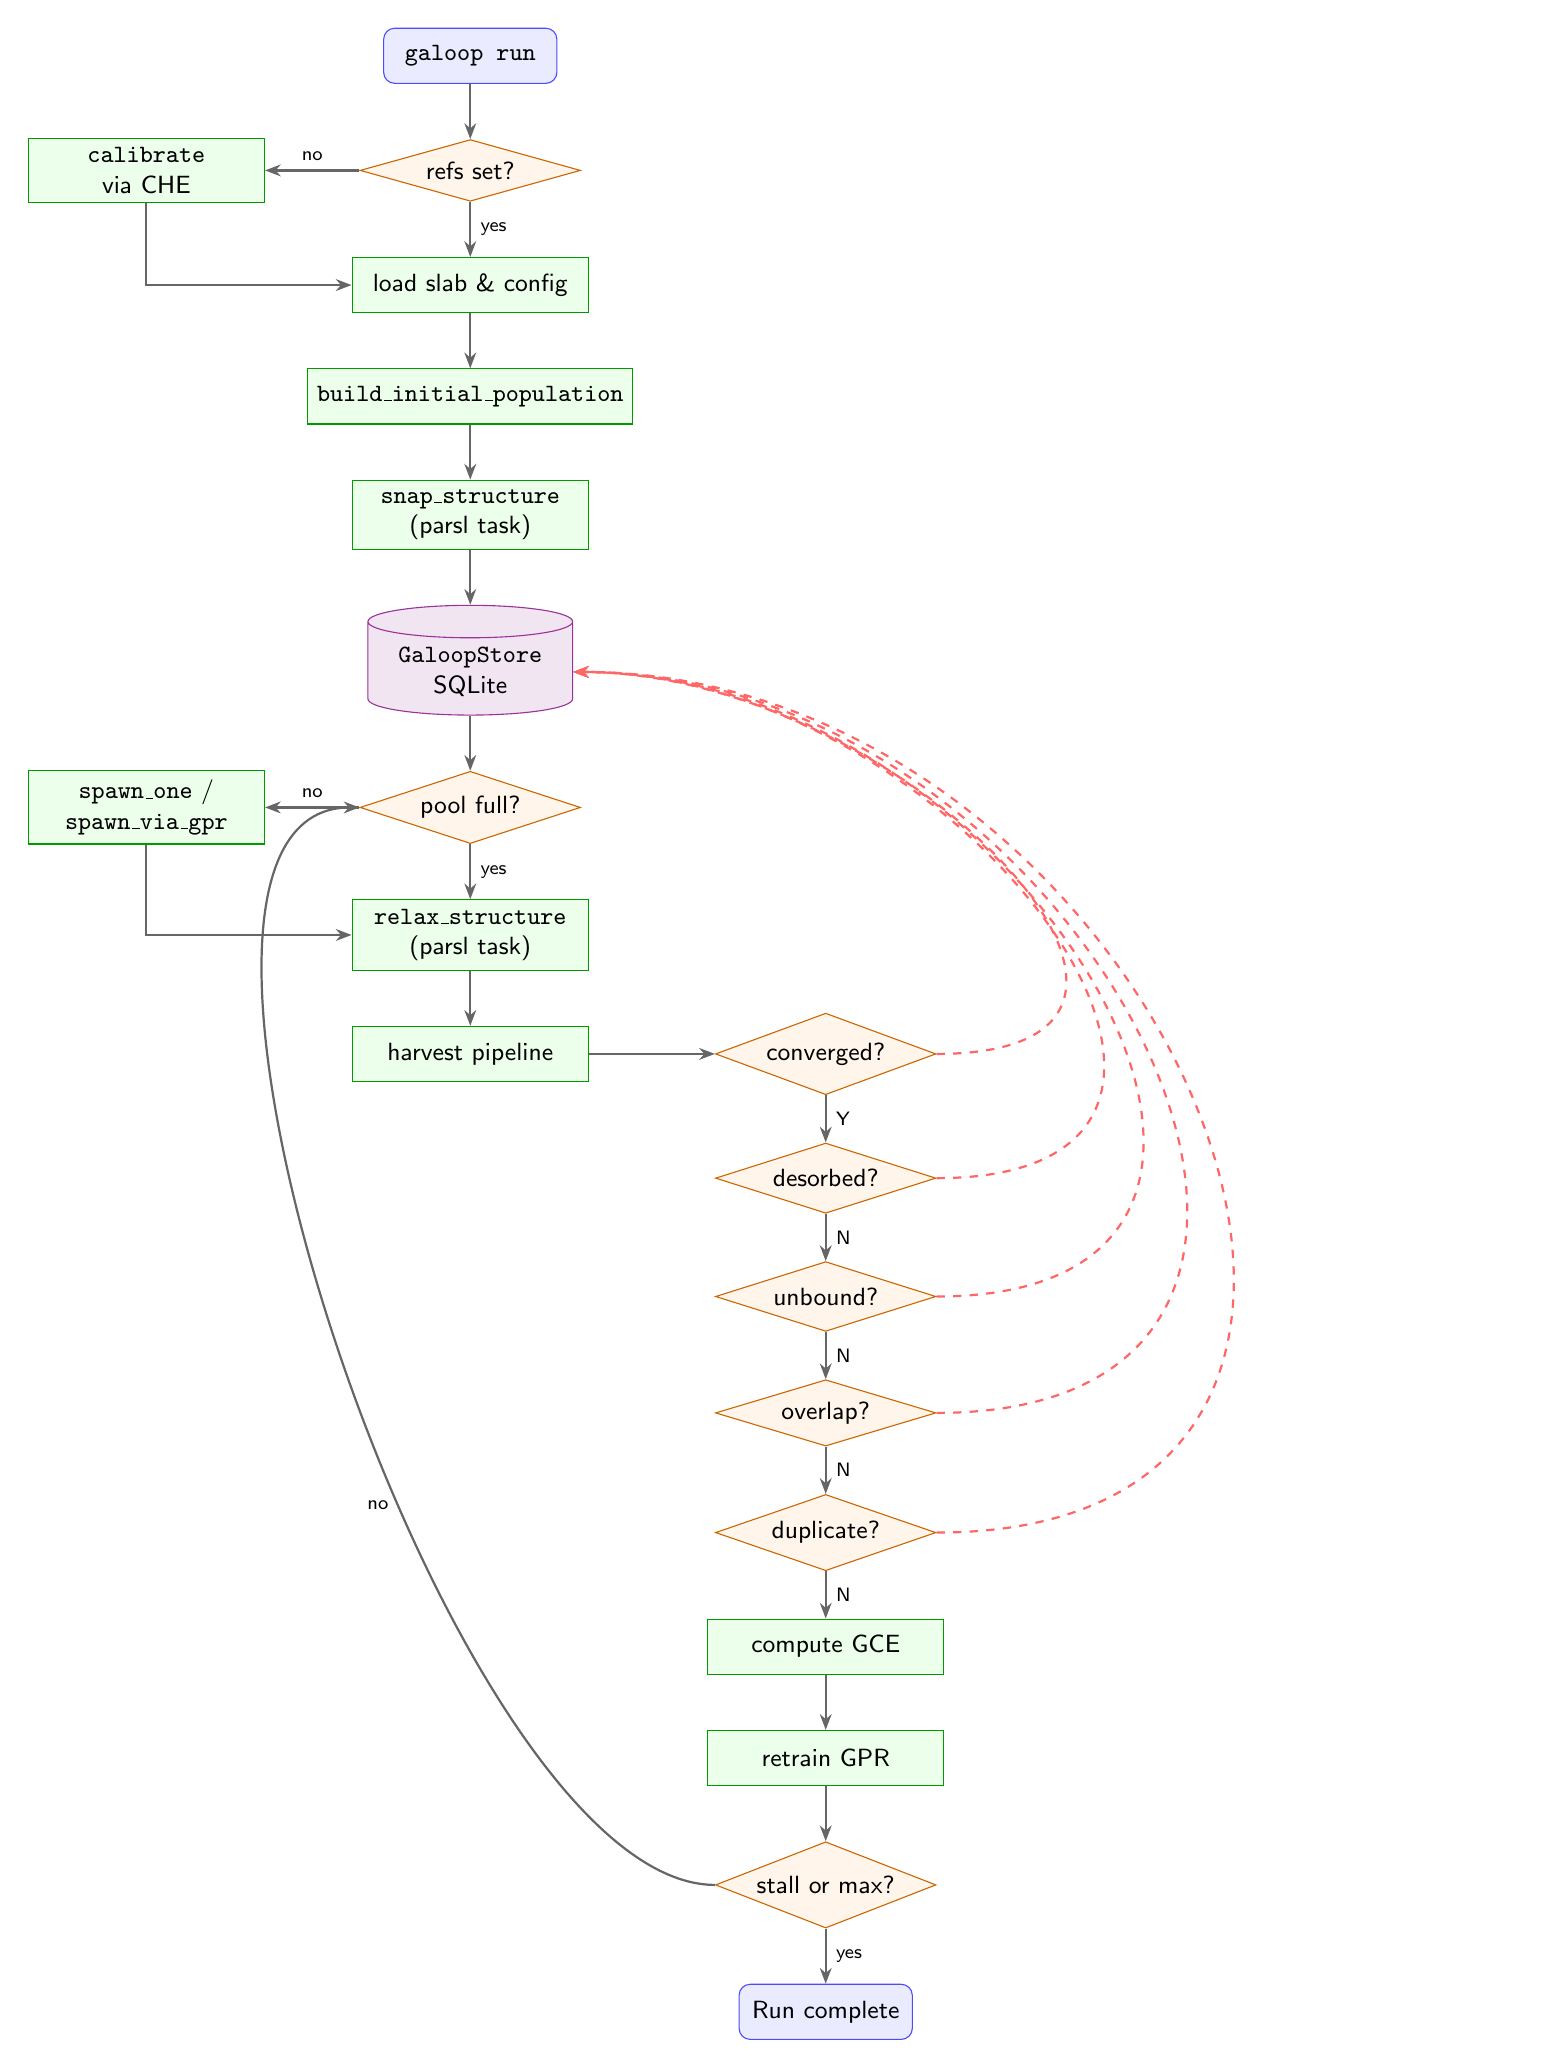
\begin{tikzpicture}[
    >={Stealth[length=2mm,width=1.5mm]},
    node distance=7mm and 9mm,
    font=\small\sffamily,
    startend/.style={rounded corners, draw=blue!70, fill=blue!8,
                     align=center, minimum width=22mm, minimum height=7mm},
    action/.style={draw=green!60!black, fill=green!8,
                   align=center, minimum width=30mm, minimum height=7mm},
    decision/.style={diamond, aspect=2, draw=orange!80!black, fill=orange!8,
                     align=center, inner sep=0pt, minimum width=28mm, minimum height=6mm},
    storage/.style={cylinder, shape border rotate=90, aspect=0.2,
                    draw=violet!80, fill=violet!10, align=center,
                    minimum width=26mm, minimum height=9mm},
    link/.style={->, thick, draw=black!60},
]

\node[startend]                         (start)    {\texttt{galoop run}};
\node[decision, below=of start]         (cal)      {refs set?};
\node[action, left=12mm of cal]         (calrun)   {\texttt{calibrate} \\ via CHE};
\node[action, below=of cal]             (loadcfg)  {load slab \& config};
\node[action, below=of loadcfg]         (initpop)  {\texttt{build\_initial\_population}};
\node[action, below=of initpop]         (snap)     {\texttt{snap\_structure} \\ (parsl task)};
\node[storage, below=of snap]           (store)    {\texttt{GaloopStore}\\SQLite};
\node[decision, below=of store]         (poll)     {pool full?};
\node[action, left=12mm of poll]        (spawn)    {\texttt{spawn\_one} / \\ \texttt{spawn\_via\_gpr}};
\node[action, below=of poll]            (relax)    {\texttt{relax\_structure} \\ (parsl task)};
\node[action, below=of relax]           (harvest)  {harvest pipeline};
\node[decision, right=16mm of harvest]  (cconv)    {converged?};
\node[decision, below=6mm of cconv]     (cdes)     {desorbed?};
\node[decision, below=6mm of cdes]      (cunb)     {unbound?};
\node[decision, below=6mm of cunb]      (cclash)   {overlap?};
\node[decision, below=6mm of cclash]    (cdup)     {duplicate?};
\node[action, below=6mm of cdup]        (cgce)     {compute GCE};
\node[action, below=of cgce]            (retrain)  {retrain GPR};
\node[decision, below=of retrain]       (stopq)    {stall or max?};
\node[startend, below=of stopq]         (done)     {Run complete};

\draw[link] (start)  -- (cal);
\draw[link] (cal)    -- node[above]{\scriptsize no} (calrun);
\draw[link] (calrun) |- (loadcfg);
\draw[link] (cal)    -- node[right]{\scriptsize yes} (loadcfg);
\draw[link] (loadcfg)-- (initpop);
\draw[link] (initpop)-- (snap);
\draw[link] (snap)   -- (store);
\draw[link] (store)  -- (poll);
\draw[link] (poll)   -- node[above]{\scriptsize no} (spawn);
\draw[link] (spawn)  |- (relax);
\draw[link] (poll)   -- node[right]{\scriptsize yes} (relax);
\draw[link] (relax)  -- (harvest);
\draw[link] (harvest)-- (cconv);
\draw[link] (cconv)  -- node[right]{\scriptsize Y} (cdes);
\draw[link] (cdes)   -- node[right]{\scriptsize N} (cunb);
\draw[link] (cunb)   -- node[right]{\scriptsize N} (cclash);
\draw[link] (cclash) -- node[right]{\scriptsize N} (cdup);
\draw[link] (cdup)   -- node[right]{\scriptsize N} (cgce);
\draw[link] (cgce)   -- (retrain);
\draw[link] (retrain)-- (stopq);
\draw[link] (stopq)  -- node[right]{\scriptsize yes} (done);
\draw[link] (stopq.west) to[out=180,in=180,looseness=0.6]
            node[left,pos=0.4]{\scriptsize no} (poll.west);

% short horizontal branches: failed classifications loop back to store
\foreach \fail in {cconv,cdes,cunb,cclash,cdup} {
    \draw[link, dashed, draw=red!60]
        (\fail.east) to[out=0,in=0,looseness=1.6] (store.east);
}

\end{tikzpicture}

\caption{End-to-end flow of a galoop campaign. Blue: entry/exit;
green: action; orange: branch; violet: persistence. Solid arrows are
the happy path; dashed red arrows show each harvest filter returning
a classified structure to the store without advancing the optimizer.
The six-stage filter (\texttt{converged?} $\to$ \texttt{desorbed?} $\to$
\texttt{unbound?} $\to$ \texttt{overlap?} $\to$ \texttt{duplicate?} $\to$
\texttt{GCE}) runs cheapest-first; each stage can short-circuit.
The canonical Mermaid source lives in \texttt{diagrams/flowchart.mmd}.}
\label{fig:flowchart}
\end{figure}

\subsection{Class architecture}

Figure~\ref{fig:uml} shows the six types that the rest of the codebase
revolves around. The intent of the drawing is to make two points that
prose obscures: first, the engine layer (\texttt{Pipeline} +
\texttt{CalculatorStage} + backend registry) has no inbound dependency
on the GA layer, so a new MLIP can be slotted in by writing a
\texttt{make\_calculator} factory and referencing it in the yaml as
\texttt{pkg.module:factory}; and second, \texttt{GaloopStore} is the
only module that touches SQLite. Everything else works through
\texttt{Individual} records and is testable without a live database.

\begin{figure}[H]
\centering
\scalebox{0.86}{
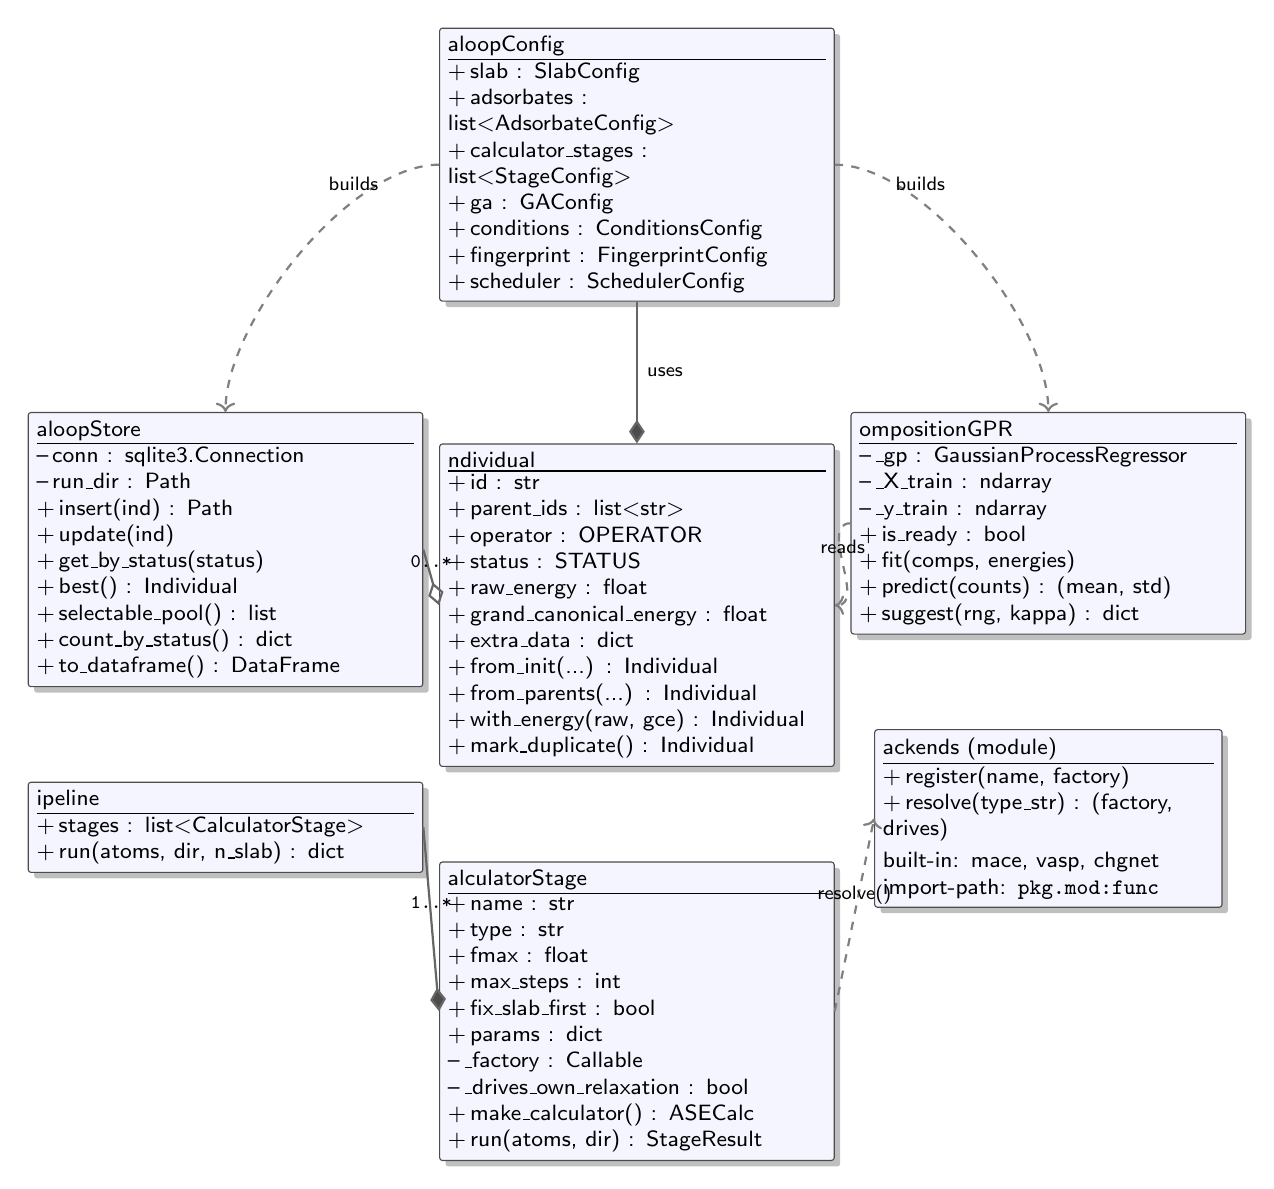
\begin{tikzpicture}[
    font=\footnotesize\sffamily,
    umlclass/.style={draw=black!70, fill=blue!4, align=left,
                     text width=48mm, inner sep=3pt,
                     rounded corners=1pt, drop shadow},
    title/.style={font=\footnotesize\bfseries},
    rel/.style={->, thick, draw=black!60},
    compose/.style={-{Diamond[length=3mm,width=2mm,fill=black!70]},
                    thick, draw=black!60},
    aggregate/.style={-{Diamond[length=3mm,width=2mm,open]},
                      thick, draw=black!60},
    dep/.style={->, thick, dashed, draw=black!50},
]

% --- Row 1: GaloopConfig (top centre) ---
\node[umlclass] (cfg) at (0,0) {
    {\title GaloopConfig}\\[1pt]
    \hrule\vspace{1pt}
    +\,slab : SlabConfig\\
    +\,adsorbates : list\textless AdsorbateConfig\textgreater\\
    +\,calculator\_stages : list\textless StageConfig\textgreater\\
    +\,ga : GAConfig\\
    +\,conditions : ConditionsConfig\\
    +\,fingerprint : FingerprintConfig\\
    +\,scheduler : SchedulerConfig
};

% --- Row 2, left: GaloopStore ---
\node[umlclass, below left=14mm and 2mm of cfg] (store) {
    {\title GaloopStore}\\[1pt]
    \hrule\vspace{1pt}
    --\,conn : sqlite3.Connection\\
    --\,run\_dir : Path\\
    +\,insert(ind) : Path\\
    +\,update(ind)\\
    +\,get\_by\_status(status)\\
    +\,best() : Individual\\
    +\,selectable\_pool() : list\\
    +\,count\_by\_status() : dict\\
    +\,to\_dataframe() : DataFrame
};

% --- Row 2, centre: Individual ---
\node[umlclass, below=18mm of cfg] (ind) {
    {\title Individual}\\[1pt]
    \hrule\vspace{1pt}
    +\,id : str\\
    +\,parent\_ids : list\textless str\textgreater\\
    +\,operator : OPERATOR\\
    +\,status : STATUS\\
    +\,raw\_energy : float\\
    +\,grand\_canonical\_energy : float\\
    +\,extra\_data : dict\\
    +\,from\_init(...) : Individual\\
    +\,from\_parents(...) : Individual\\
    +\,with\_energy(raw, gce) : Individual\\
    +\,mark\_duplicate() : Individual
};

% --- Row 2, right: CompositionGPR ---
\node[umlclass, below right=14mm and 2mm of cfg] (gpr) {
    {\title CompositionGPR}\\[1pt]
    \hrule\vspace{1pt}
    --\,\_gp : GaussianProcessRegressor\\
    --\,\_X\_train : ndarray\\
    --\,\_y\_train : ndarray\\
    +\,is\_ready : bool\\
    +\,fit(comps, energies)\\
    +\,predict(counts) : (mean, std)\\
    +\,suggest(rng, kappa) : dict
};

% --- Row 3: Pipeline and CalculatorStage ---
\node[umlclass, below=12mm of store] (pipe) {
    {\title Pipeline}\\[1pt]
    \hrule\vspace{1pt}
    +\,stages : list\textless CalculatorStage\textgreater\\
    +\,run(atoms, dir, n\_slab) : dict
};

\node[umlclass, below=12mm of ind] (stage) {
    {\title CalculatorStage}\\[1pt]
    \hrule\vspace{1pt}
    +\,name : str\\
    +\,type : str\\
    +\,fmax : float\\
    +\,max\_steps : int\\
    +\,fix\_slab\_first : bool\\
    +\,params : dict\\
    --\,\_factory : Callable\\
    --\,\_drives\_own\_relaxation : bool\\
    +\,make\_calculator() : ASECalc\\
    +\,run(atoms, dir) : StageResult
};

\node[umlclass, below=12mm of gpr, text width=42mm] (bk) {
    {\title backends (module)}\\[1pt]
    \hrule\vspace{1pt}
    +\,register(name, factory)\\
    +\,resolve(type\_str) : (factory, drives)\\[2pt]
    built-in: mace, vasp, chgnet\\
    import-path: \texttt{pkg.mod:func}
};

% --- relationships ---
\draw[compose]  (cfg.south) -- (ind.north) node[pos=0.5,right]{\scriptsize uses};
\draw[aggregate] (store.east) -- (ind.west) node[pos=0.5,above]{\scriptsize \tt 0..*};
\draw[compose]   (pipe.east) -- (stage.west) node[pos=0.5,above]{\scriptsize \tt 1..*};
\draw[dep]       (stage.east) -- (bk.west) node[pos=0.5,above]{\scriptsize resolve()};
\draw[dep]       (gpr.west) to[out=180,in=0] node[above,pos=0.5]{\scriptsize reads} (ind.east);
\draw[dep]       (cfg.west) to[out=180,in=90,looseness=0.7]
                 node[above,pos=0.3]{\scriptsize builds}  (store.north);
\draw[dep]       (cfg.east) to[out=0,in=90,looseness=0.7]
                 node[above,pos=0.3]{\scriptsize builds}  (gpr.north);

\end{tikzpicture}
}

\caption{Core class diagram of galoop. Filled diamonds denote
composition (\texttt{GaloopConfig} owns its sub-configs;
\texttt{Pipeline} owns its \texttt{CalculatorStage}s); open diamonds
denote aggregation (\texttt{GaloopStore} persists, but does not own,
\texttt{Individual}s); dashed arrows denote usage dependencies. The
\texttt{backends} module is a small registry with two built-ins
(\texttt{mace}, \texttt{vasp}, \texttt{chgnet}) plus dynamic
resolution of any \texttt{pkg.module:factory} import path — this is
the extension point for bringing your own MLIP. Canonical Mermaid
source at \texttt{diagrams/uml.mmd}.}
\label{fig:uml}
\end{figure}

\subsection{Harvest pipeline detail}

Every future that comes back from a Parsl \texttt{relax\_structure}
call is passed through a six-stage classifier in
\texttt{galoop/harvest.py}, in strict cheapest-first order:

\begin{enumerate}
  \item \textbf{Convergence}: did BFGS reach \texttt{fmax}, and is the
    final energy finite?
  \item \textbf{Desorption}: any adsorbate atom more than
    $z_{\max}+3$\,\AA{} above the slab top?
  \item \textbf{Surface binding}: every adsorbate \emph{molecule}
    (grouped via covalent radii in
    \texttt{\_group\_molecules}) has at least one atom within
    $1.3\times$covalent-radii of a slab atom.
  \item \textbf{Atom overlap}: no two atoms closer than 0.5\,\AA{}.
  \item \textbf{Fingerprint cascade}: composition gate $\to$ energy
    gate $\to$ distance-histogram cosine pre-filter $\to$
    SOAP-Tanimoto against the accumulated cache.
  \item \textbf{GCE}: compute $G$ from Equation~\ref{eq:gce}, insert
    into the cache, and return the updated best.
\end{enumerate}

Stages~1--5 short-circuit: a structure that fails at \texttt{desorbed}
never touches SOAP. In practice the first two stages reject the bulk
of the volume on weakly-binding metals
(Section~\ref{sec:physics-reproductions}).

\subsection{Parsl dispatch and log rotation}

Both \texttt{snap\_structure} (init-pop constrained pre-relax) and
\texttt{relax\_structure} (full pipeline) are
\texttt{@python\_app}-decorated Parsl tasks
(\texttt{galoop/engine/scheduler.py}). Dispatching snap through Parsl
rather than running it in-process means the main galoop process
never has to load the MLIP, which matters on tight-GPU machines where
the main process and the worker would otherwise contend for the same
memory.

One infrastructure pain point the validation sweep surfaced was that
Parsl's HTEX workers write their \texttt{manager.log} via a plain
\texttt{FileHandler} with no bound. Workers that survive their parent
process (after a kill, segfault, or pytest interruption) keep writing
forever; by the end of a long session the 2026-04-09 sweep machine
had 18 orphaned workers holding multi-GB log files open on disk, one
at 6.7~GB. Galoop now monkey-patches
\texttt{parsl.log\_utils.set\_file\_logger} to install a
\texttt{RotatingFileHandler} with a 50~MiB cap and 3 rotated backups
(tunable via \texttt{GALOOP\_PARSL\_LOG\_MAX\_BYTES} and
\texttt{GALOOP\_PARSL\_LOG\_BACKUPS}). The patch is installed both
in the main process (via a side-effect import at the top of
\texttt{engine/scheduler.py}) and in each worker subprocess (by
overriding the HTEX launch command to invoke a wrapper module that
reinstalls the patch before forwarding to Parsl's real worker entry
point via \texttt{runpy}). Worst-case per-worker on-disk footprint is
now $50\,\text{MiB}\,\times\,(1+3) = 200$\,MiB instead of unbounded.

% ============================================================================
\section{Validation sweep}
\label{sec:sweep}

To stress-test the pipeline after two recent refactors (pluggable
backend factory, non-orthogonal surface normals) we ran a
ten-campaign sweep across the catalytic-metal zoo. Every campaign used
the same MLIP backend — FAIRChem UMA (\texttt{uma-s-1p1},
\texttt{oc20} task) on CUDA — via the import-path factory
\texttt{calc:make\_calculator} in each run directory. Common GA
settings: \texttt{population\_size: 20}, \texttt{max\_structures: 450},
\texttt{max\_stall: 40} (early runs) or \texttt{15} (later runs),
\texttt{duplicate\_threshold: 0.88}, single Parsl worker,
\texttt{gpr\_guided: true}. Total wall clock: $\sim$6~h~20~m.

\subsection{Campaigns}

\begin{table}[H]
\centering\small
\begin{tabular}{@{}lllcrrrr@{}}
\toprule
\# & Metal/facet & Adsorbates & $U$ (V) & Runtime & conv.\ & yield & $G_{\min}$ (eV) \\
\midrule
1  & Cu(111) fcc  & CO/H/H$_2$O           &  0.0 &  17 min &  13 &  8\%   & $-397.64$ \\
2  & Cu(100) fcc  & CO/H/H$_2$O           &  0.0 &  67 min &  24 & 10\%   & $-450.11$ \\
3  & Cu(211) fcc  & CO/H/H$_2$O           &  0.0 &  19 min &  14 & 10\%   & $-435.78$ \\
4  & Pt(111) fcc  & O/OH/OOH/H            &  0.8 &  33 min &  32 & 17\%   & $-481.32$ \\
5  & Pt(211) fcc  & N/NH/NH$_2$/NH$_3$/H  & $-0.5$ & 74 min  &  23 & 11\%   & $-459.68$ \\
6  & Ag(111) fcc  & CO/H/H$_2$O           &  0.0 &  32 min &   9 & \textbf{3.5\%} & $-218.49$ \\
7  & Pd(111) fcc  & H                      &  0.0 &  \textbf{8 min} & 16 & 20\%   & $-322.47$ \\
8  & Ni(111) fcc  & C/CH/CH$_2$/CH$_3$/H  &  0.0 &  20 min &  26 & 21\%   & $-514.93$ \\
9  & Au(111) fcc  & CO/OH                 &  0.0 &  80 min &  16 &  4.3\% & $-296.04$ \\
10 & Ru(0001) hcp & O/OH/H$_2$O           &  0.0 &  12 min &  13 &  9\%   & \textbf{$-581.99$} \\
\bottomrule
\end{tabular}
\caption{Summary of the ten validation campaigns. "Conv." is the
number of converged structures at termination; "yield" is
conv./attempts. Several runs were stopped early via
\texttt{galoopstop} when stall-grinding became unproductive; all
produced a usable $G_{\min}$.}
\label{tab:summary}
\end{table}

\subsection{Best structures}

Figure~\ref{fig:structs} shows the lowest-$G$ configuration from each
campaign, rendered top-down (left half of each pair) and profile (right
half) with \texttt{ase.visualize.plot.plot\_atoms}. These are the
physical answers to what the GA asked at each $(U, \text{pH})$.

\begin{figure}[H]
  \centering
  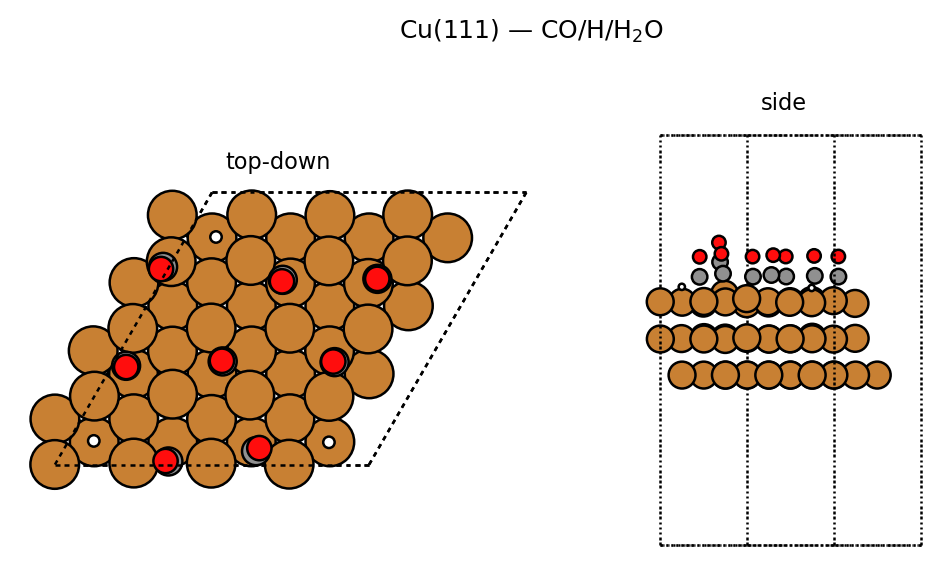
\includegraphics[width=0.245\textwidth]{struct_cu111_co_camp.png}\hfill
  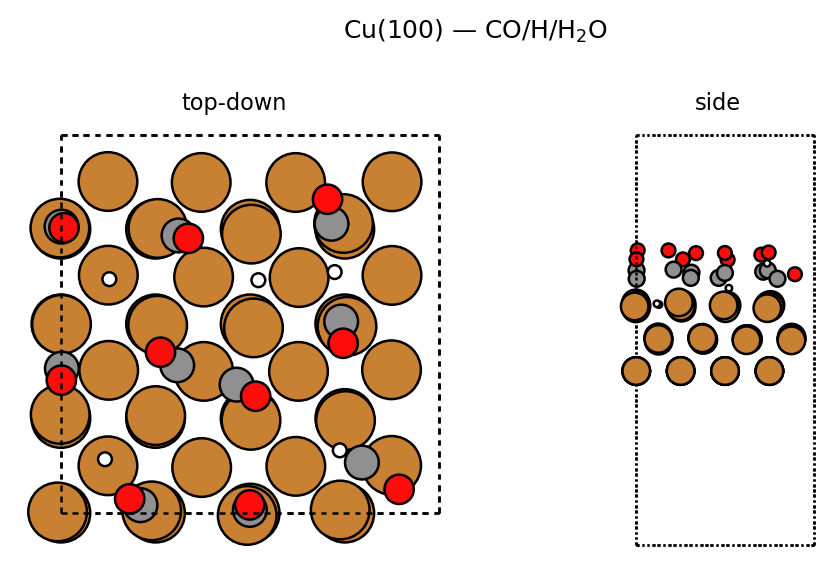
\includegraphics[width=0.245\textwidth]{struct_cu100_co_camp.png}\hfill
  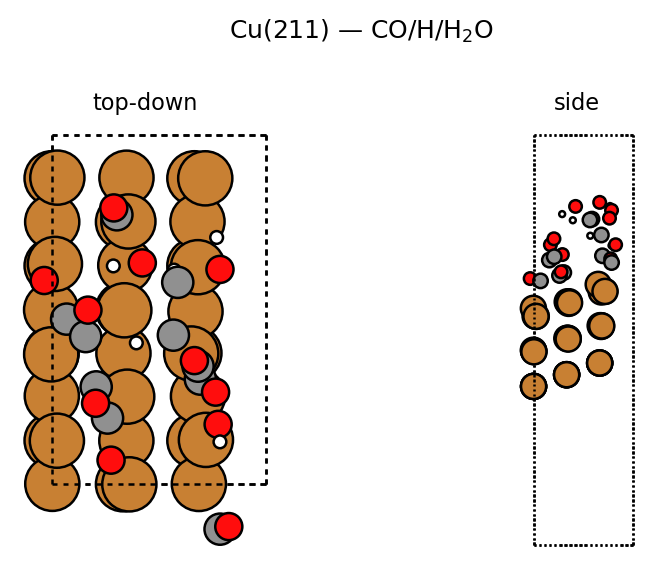
\includegraphics[width=0.245\textwidth]{struct_cu211_co_camp.png}\hfill
  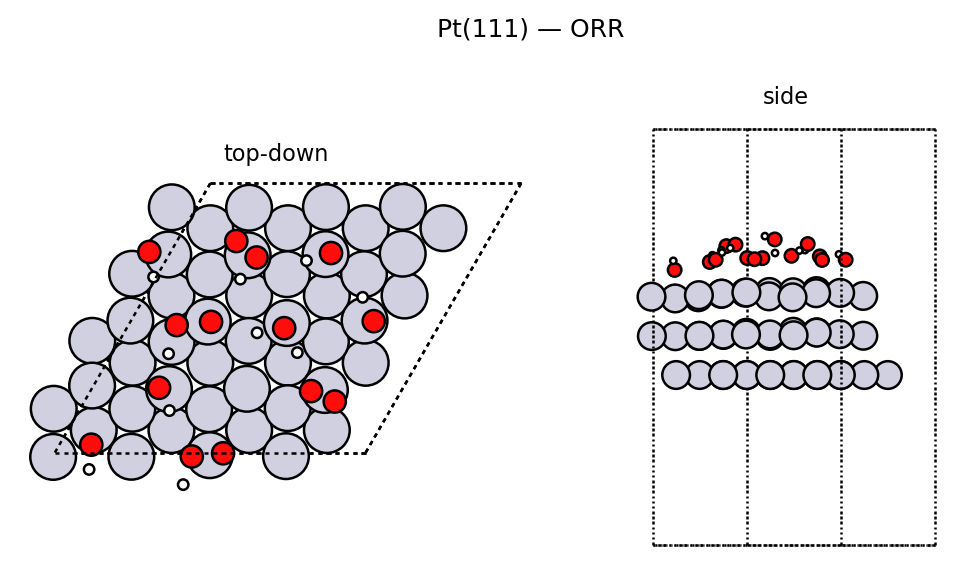
\includegraphics[width=0.245\textwidth]{struct_pt111_orr_camp.png}\\[0.4em]
  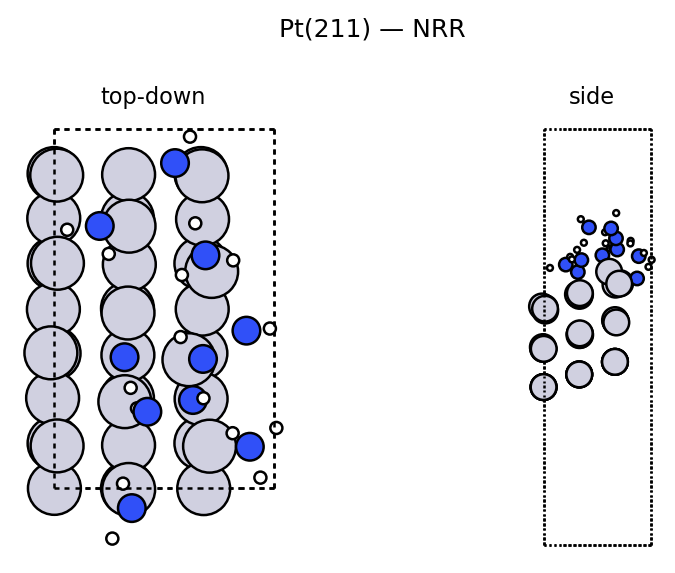
\includegraphics[width=0.245\textwidth]{struct_pt211_nrr_camp.png}\hfill
  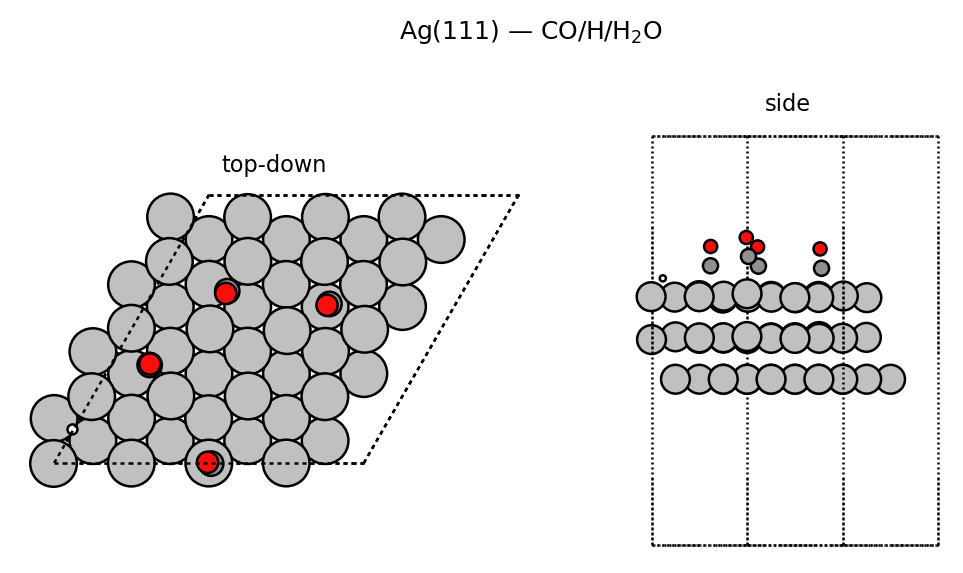
\includegraphics[width=0.245\textwidth]{struct_ag111_co_camp.png}\hfill
  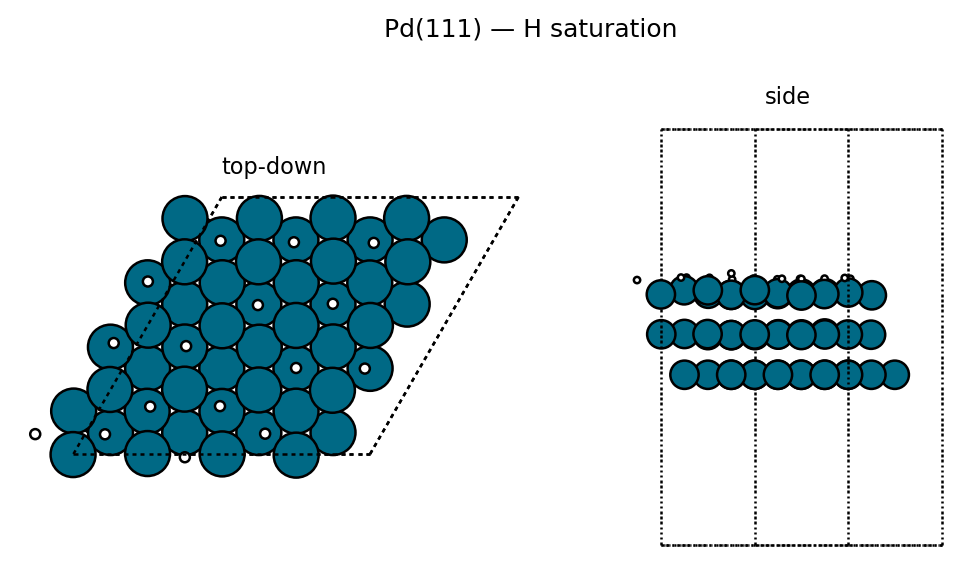
\includegraphics[width=0.245\textwidth]{struct_pd111_hsat_camp.png}\hfill
  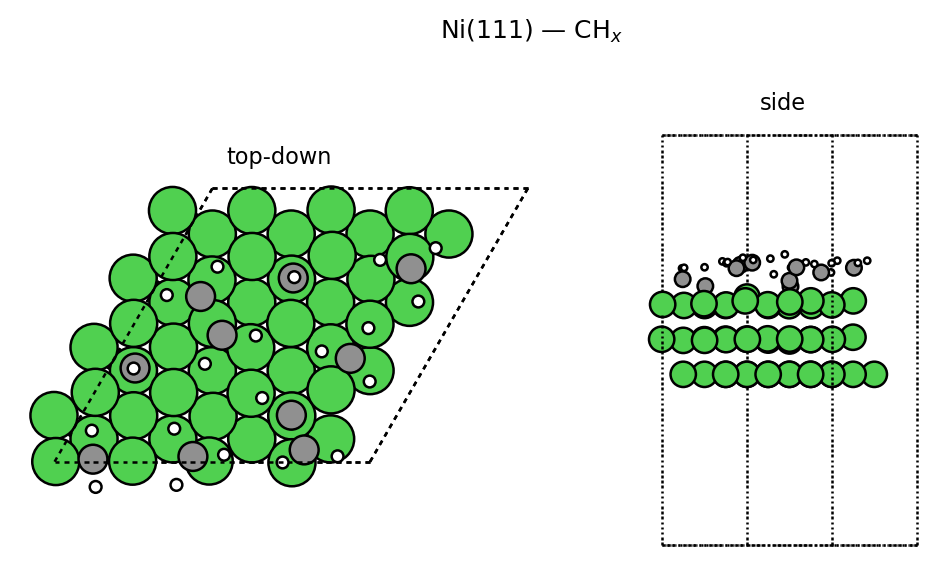
\includegraphics[width=0.245\textwidth]{struct_ni111_chx_camp.png}\\[0.4em]
  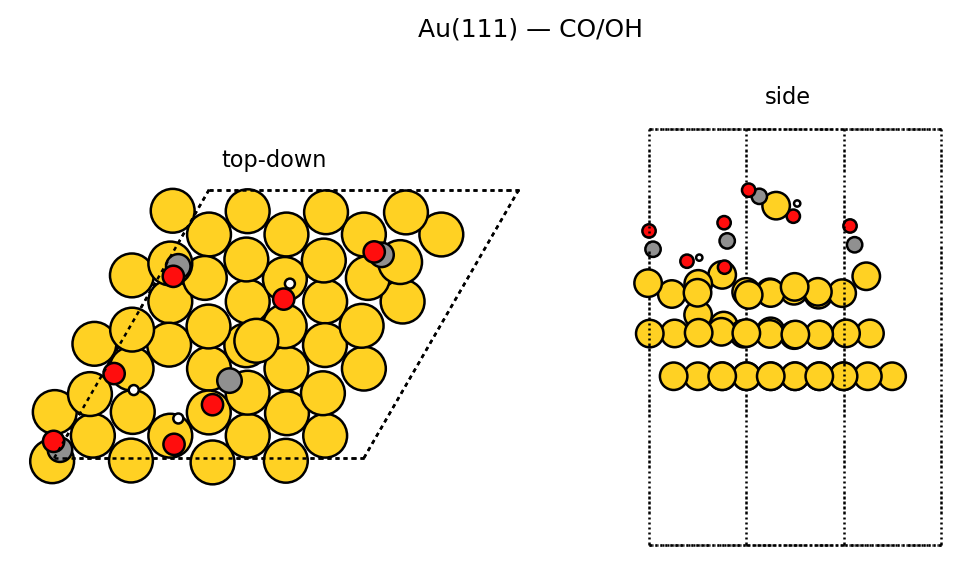
\includegraphics[width=0.245\textwidth]{struct_au111_co_camp.png}\hfill
  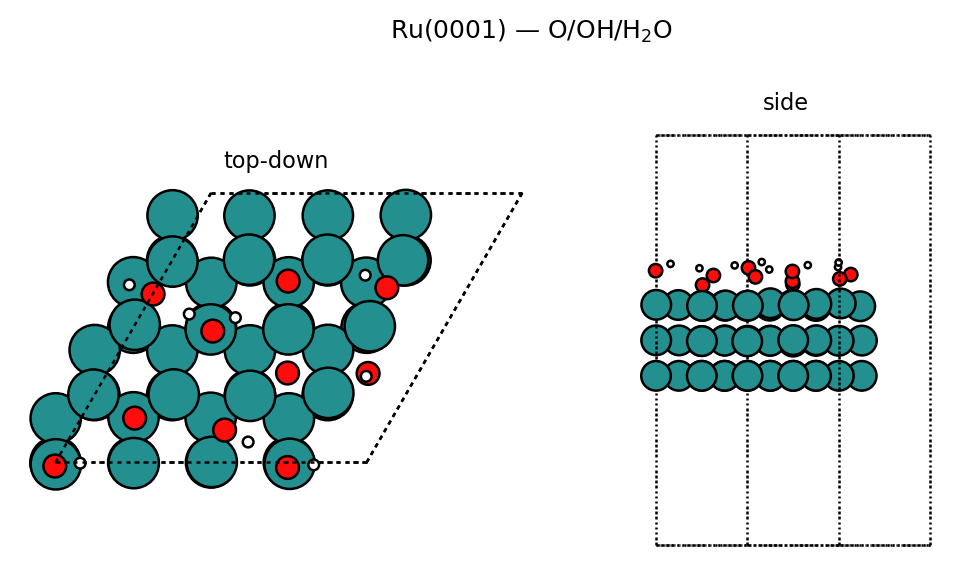
\includegraphics[width=0.245\textwidth]{struct_ru0001_oh_camp.png}

  \caption{Lowest-$G$ structures from each campaign. Reading order:
  Cu(111), Cu(100), Cu(211), Pt(111)-ORR, Pt(211)-NRR, Ag(111),
  Pd(111)-H saturation, Ni(111)-CH$_x$, Au(111), Ru(0001). Each tile
  shows the same structure top-down (left) and profile (right).}
  \label{fig:structs}
\end{figure}

\subsection{Duplicate detection performance}
\label{sec:dup-perf}

Figure~\ref{fig:heatmap} projects every adsorbate atom from every
converged structure onto the fractional ($a$, $b$) basis of the slab
cell. Bright regions are where the GA actually placed things; dark
regions are unexplored. The hexagonal arrangement of fcc(111) atop
sites shows up clearly on Cu, Pd, Ni, Ag; Pd(111)-H saturates
uniformly at 1~ML; the Cu(211) and Pt(211) stepped facets show the
characteristic narrow-stripe pattern along the step-edge direction.

\begin{figure}[H]
  \centering
  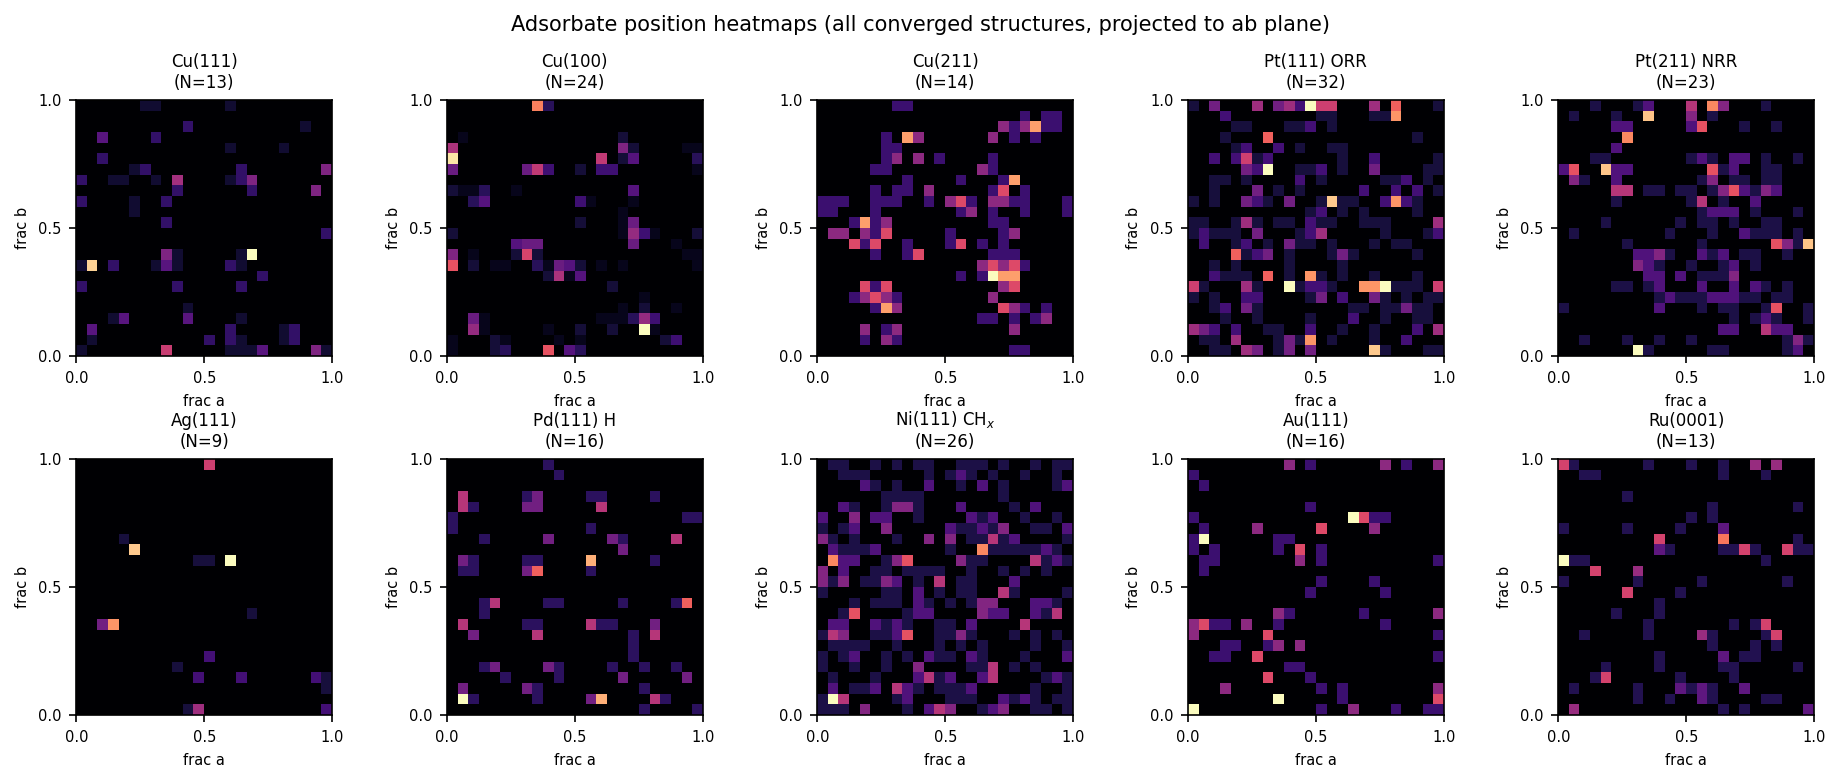
\includegraphics[width=\linewidth]{heatmap_grid.png}
  \caption{Adsorbate-position heatmaps per campaign. For each run we
  pool the fractional ($a$, $b$) positions of every adsorbate atom
  from every converged structure and 2D-histogram them into 24$\times$24
  bins. $N$ in each title is the number of converged structures
  contributing. The stepped facets (Cu(211), Pt(211)) show their
  characteristic stripes along the periodic-step direction.}
  \label{fig:heatmap}
\end{figure}

Figure~\ref{fig:rdf} shows the pooled adsorbate--adsorbate pair
distance distributions. Intra-molecular peaks in the 1--1.5~\AA{}
range (C$=$O, O$-$H, N$-$H bonds) are visible on most runs, and the
3--5~\AA{} band is surface nearest-neighbours. Ag and Au are notably
sparse past 2\,\AA{} because they converged so few structures.

\begin{figure}[H]
  \centering
  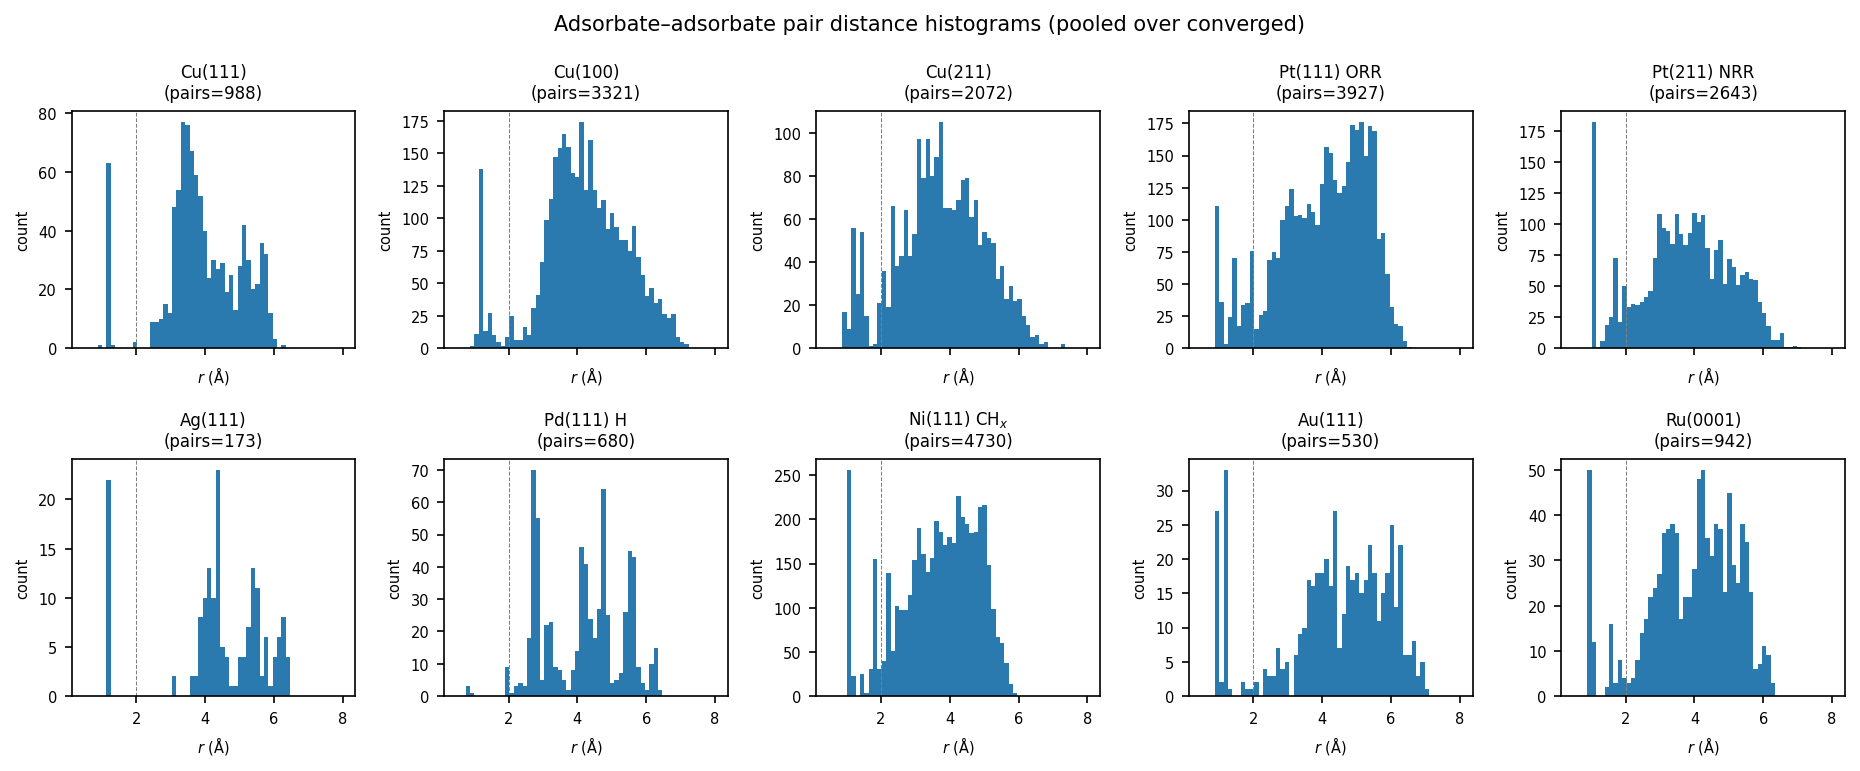
\includegraphics[width=\linewidth]{rdf_grid.png}
  \caption{Adsorbate--adsorbate pair-distance histograms pooled over
  converged structures, per campaign. Dashed vertical line at 2.0~\AA{}
  marks the atom-overlap rejection threshold. Intra-molecular bond
  lengths sit below 1.5~\AA{} and site-to-site nearest-neighbour
  distances are in the 3--5~\AA{} range.}
  \label{fig:rdf}
\end{figure}

\paragraph{SOAP cutoff sensitivity.}
A legitimate concern with any SOAP-based duplicate detector is that
the call is dominated by the choice of cutoff. We probed that by
computing the all-pairs similarity matrix of every converged
structure in three representative campaigns
(Cu(111), Pd(111)-H, Ru(0001)) under five different
$(r_{\text{cut}}, n_{\max}, l_{\max})$ settings, and plotting the
fraction of pairs whose similarity exceeds a given threshold
(Fig.~\ref{fig:soap-curves}). The curves bundle tightly near the
default threshold $\tau=0.92$ on Pd(111)-H (single-species, low
internal complexity) and fan out more on Cu(111) and Ru(0001)
(adsorbate-rich), but never swap their ordering.

\begin{figure}[H]
  \centering
  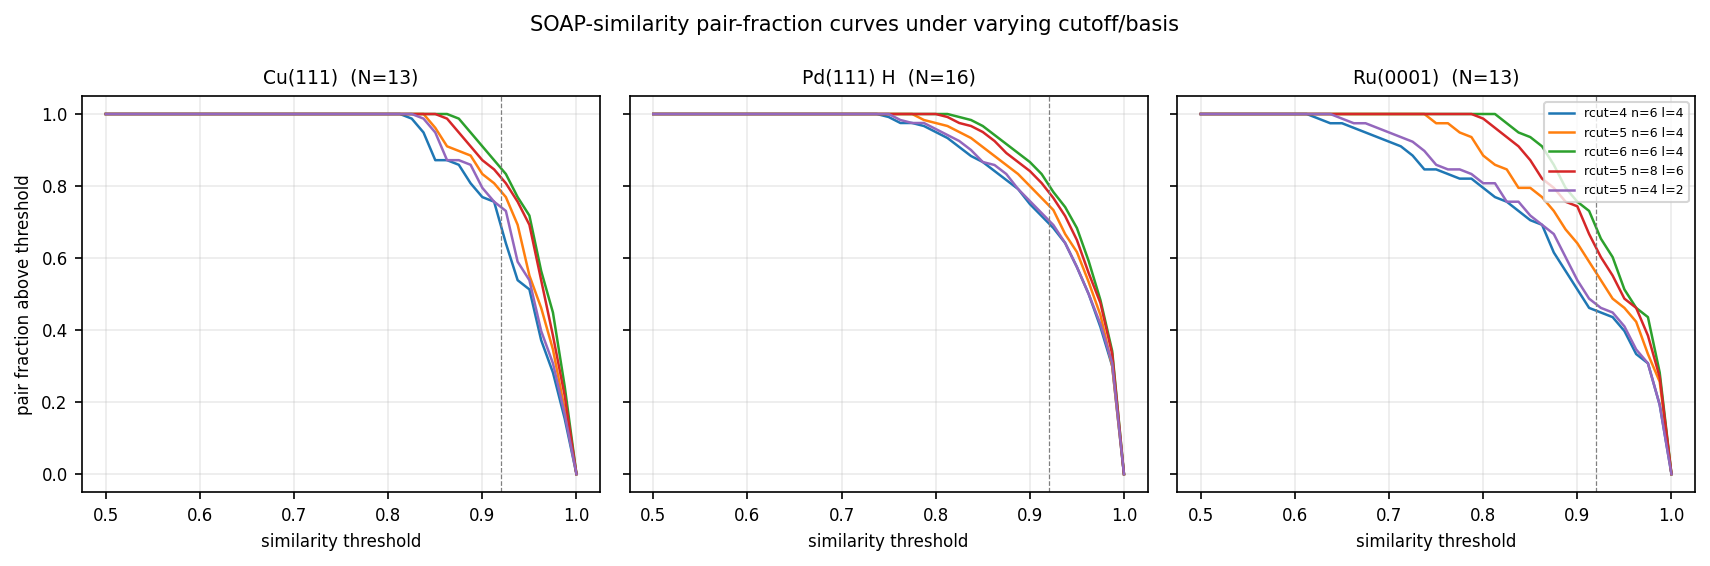
\includegraphics[width=\linewidth]{soap_dup_curves.png}
  \caption{Fraction of adsorbate-pair SOAP similarities exceeding a
  given threshold for five $(r_{\text{cut}}, n_{\max}, l_{\max})$
  settings, evaluated on the converged-structure pool of three
  campaigns. The dashed vertical line is galoop's default threshold
  of 0.92. Curves cluster tightly near the threshold, meaning the
  pairwise duplicate verdict is essentially invariant to cutoff
  choice in the typical 4--6~\AA{} range.}
  \label{fig:soap-curves}
\end{figure}

\begin{figure}[H]
  \centering
  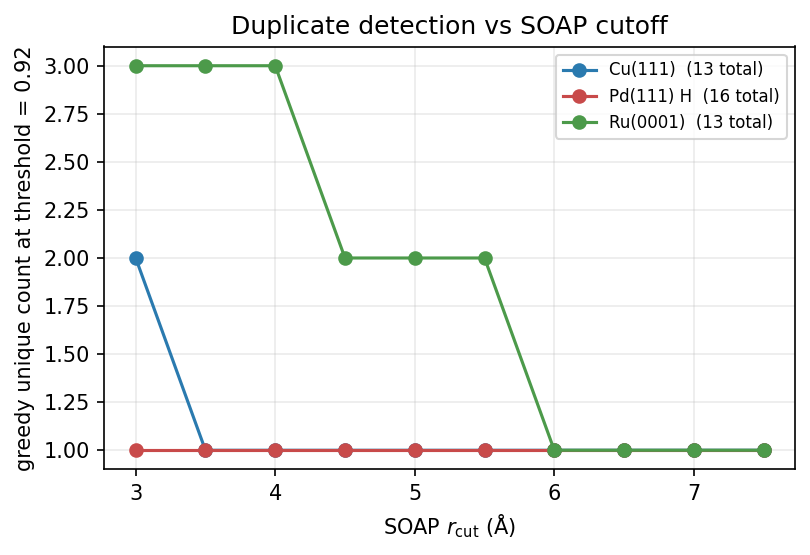
\includegraphics[width=0.62\linewidth]{soap_rcut_unique.png}
  \caption{Greedy unique-structure count at a fixed similarity
  threshold of 0.92, as a function of $r_{\text{cut}}$. A plateau
  across the 4--7~\AA{} range on Cu(111) and Ru(0001) means the
  duplicate call is robust to shifts in cutoff inside the band
  actually used in practice. Pd(111)-H is essentially flat because
  the single-species search space is small.}
  \label{fig:soap-rcut}
\end{figure}

The takeaway is in the \texttt{keyfindings} box below: duplicate
detection on this data is a stable operation. The tuning pain that
high pre-relax duplicate rates cause (bug~6 in our list) is not about
choosing the right SOAP parameters but about the GA exhausting small
composition basins quickly.

\begin{keyfindings}[Duplicate detection is cutoff-robust]
Across the tested 4--7~\AA{} $r_{\text{cut}}$ range, the greedy unique
count changes by no more than 1--2 structures on any campaign with
$\geq 13$ converged entries. The SOAP-Tanimoto gate is therefore
effectively a fixed classifier under routine tuning, and the 90\%+
duplicate rates observed in small-search-space campaigns (Cu(111),
Ag(111)) reflect saturation of the compositional landscape, not
fingerprint mis-calls.
\end{keyfindings}

\subsection{GPR guidance analysis}
\label{sec:gpr-results}

Figure~\ref{fig:op-counts} breaks down the converged population of
each campaign by the operator that produced it. GPR (red) dominates
on Pt(111)-ORR and Ni(111)-CH$_x$, where the composition landscape is
richest and the surrogate has enough dimensions to exploit; it is
nearly absent from the Cu runs, because \texttt{init} placement found
the optimum before GPR reached its \texttt{gpr\_min\_samples}
activation threshold.

\begin{figure}[H]
  \centering
  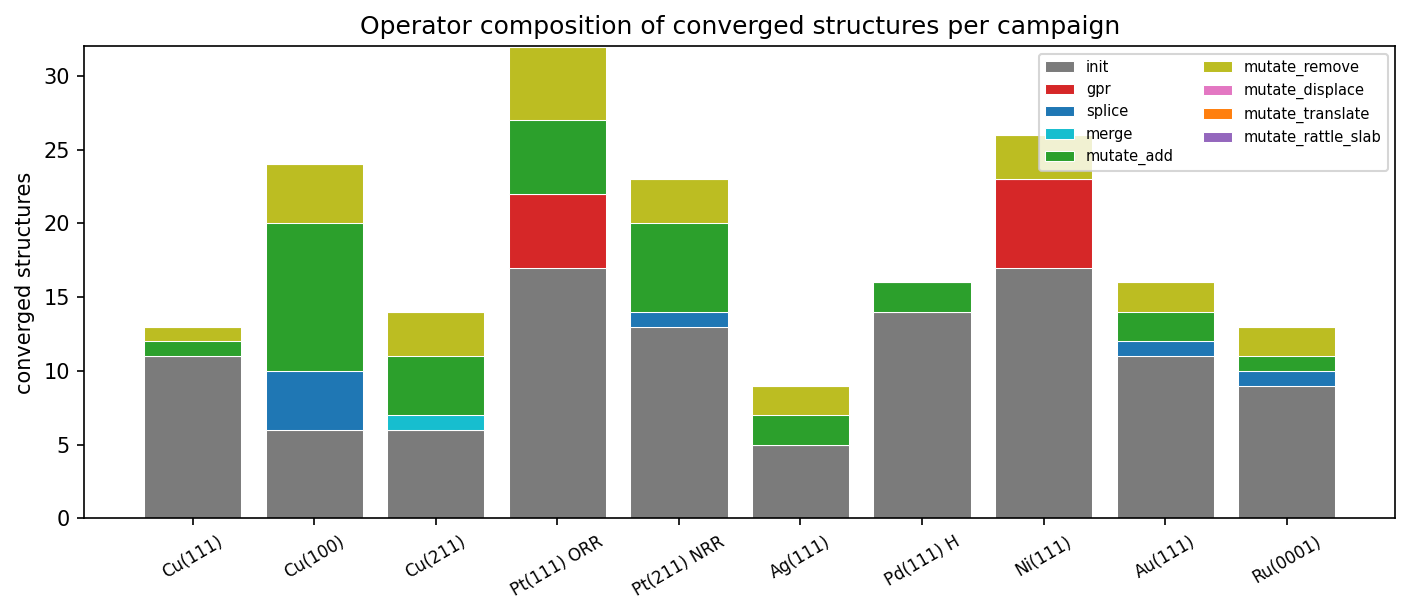
\includegraphics[width=\linewidth]{operator_counts.png}
  \caption{Stacked count of converged structures per campaign, by
  producing operator. Grey: \texttt{init} placement; red: GPR
  surrogate; blue/cyan/green shades: GA crossover and mutation
  operators. The heavier the red band, the more the GPR thinks it
  has a handle on the composition--energy relationship.}
  \label{fig:op-counts}
\end{figure}

Figure~\ref{fig:gevo} plots the grand canonical energy of each
converged structure against its discovery order, colored by operator.
The dashed black line is the running minimum. In Pt(111)-ORR and
Ni(111)-CH$_x$ the running best is defined by GPR points; in Cu(111)
the running best sits on an \texttt{init} point the GA never
improved upon.

\begin{figure}[H]
  \centering
  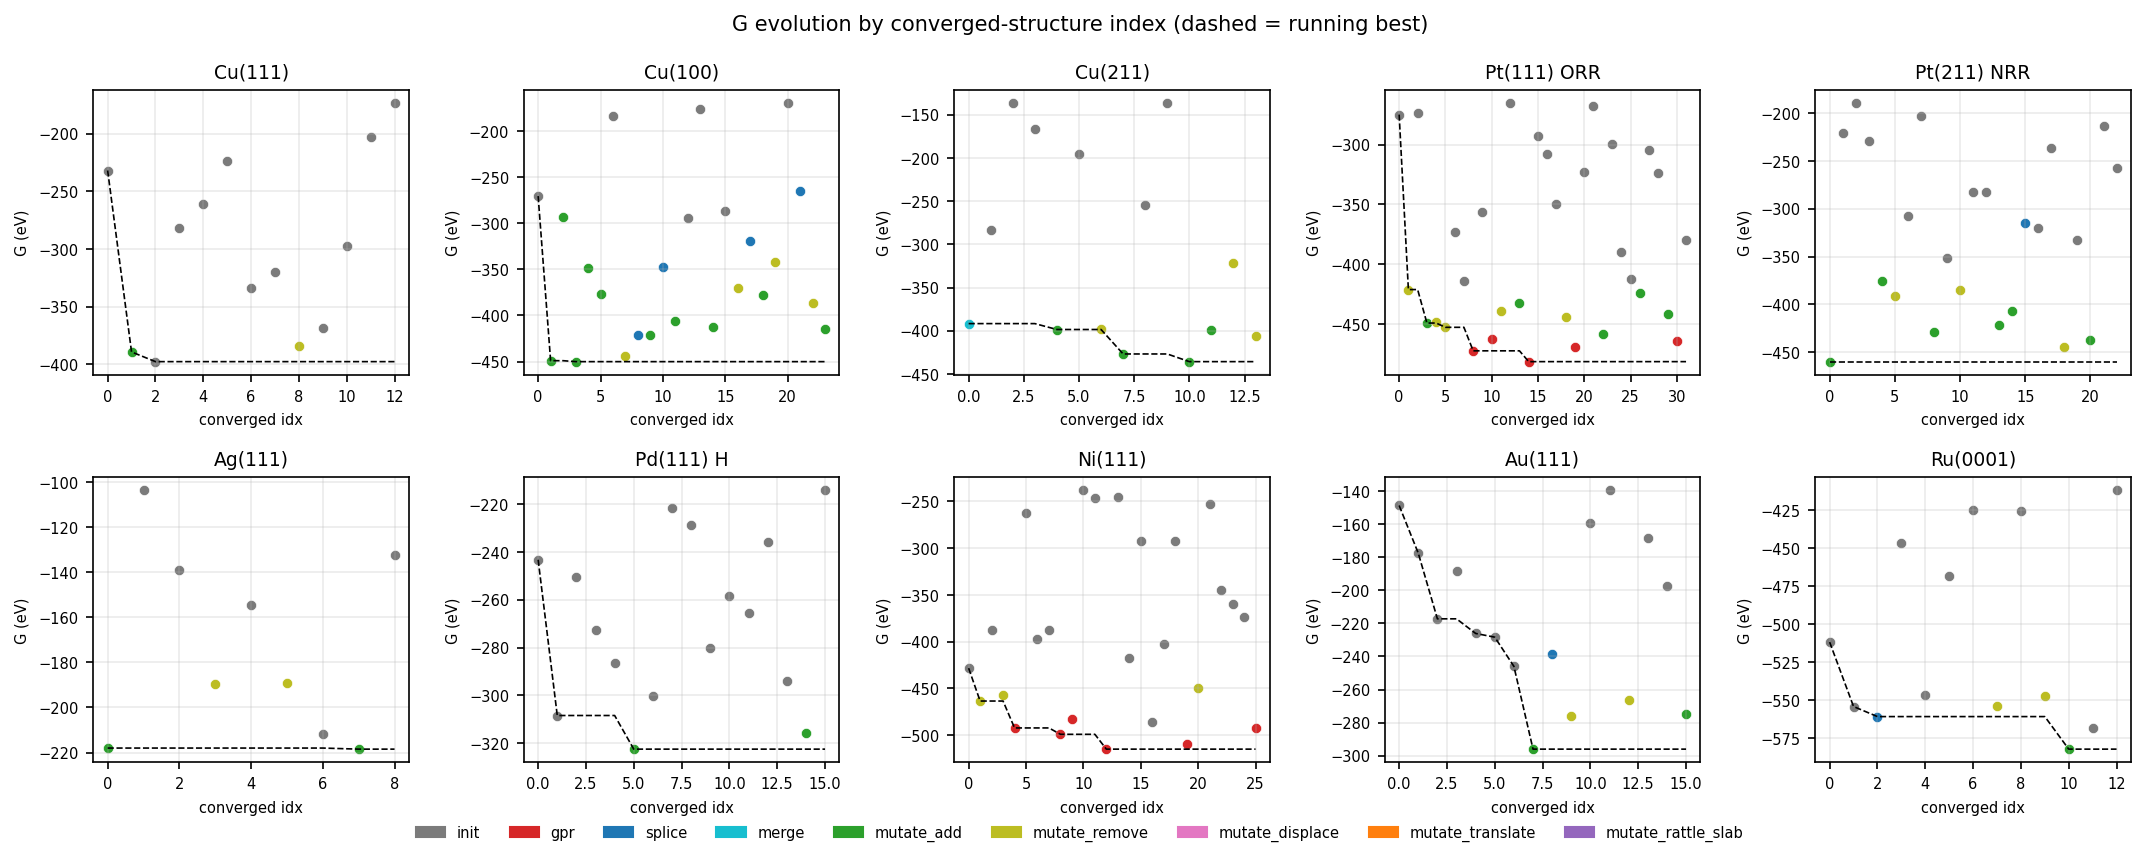
\includegraphics[width=\linewidth]{g_evolution.png}
  \caption{Grand canonical energy vs converged-structure discovery
  order, per campaign. Dashed: running minimum. Points are coloured
  by the operator that produced them — legend at the bottom.}
  \label{fig:gevo}
\end{figure}

A more compact view of the same question: Figure~\ref{fig:gprbox}
shows the per-campaign $G$-distribution for GPR-spawned converged
structures vs.\ everything else. When the GPR box sits below the
non-GPR box, the surrogate is steering toward strictly better basins.

\begin{figure}[H]
  \centering
  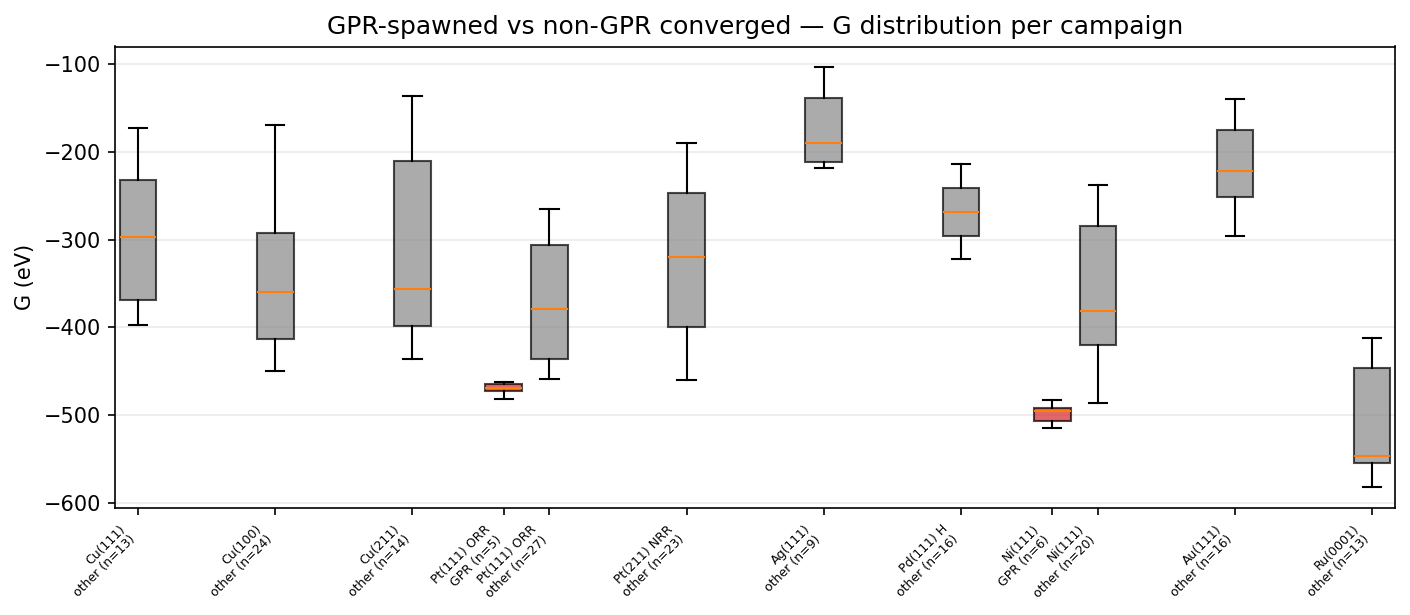
\includegraphics[width=\linewidth]{gpr_vs_nongpr_box.png}
  \caption{Per-campaign $G$ distribution for GPR-proposed converged
  structures (red) versus everything else (grey). Missing boxes
  indicate the GPR never activated on that run. On Pt(111)-ORR,
  Pt(211)-NRR, and Ni(111)-CH$_x$ the GPR median sits below the
  non-GPR median; on Cu(111) GPR is absent from the top.}
  \label{fig:gprbox}
\end{figure}

\paragraph{Where GPR helps, where it misleads.}

\noindent\begin{tcolorbox}[colback=lightgreen, colframe=sciencegreen,
  fonttitle=\bfseries\color{white}, title=Three observed GPR regimes,
  coltitle=white, colbacktitle=sciencegreen,
  boxrule=1pt, arc=3pt, left=8pt, right=8pt, top=6pt, bottom=6pt,
  before skip=12pt, after skip=12pt,
  grow to left by=0pt, grow to right by=0pt]
\sloppy\small
\textbf{Helpful regime.} Pt(111)-ORR and Ni(111)-CH$_x$ have 4--5
species — enough composition dimensions for the Mat{\'e}rn kernel to
learn a meaningful surface. GPR proposals steer directly into
saturation-level OH/OOH and CH$_2$/CH$_3$ mixtures that the GA
operators would only reach by many splice/merge cycles.

\medskip\noindent
\textbf{Irrelevant regime.} Cu(111) with CO/H/H$_2$O has a search
space small enough that \texttt{init} placement alone hit the optimum
before GPR collected its training-data threshold. GPR activated but
never contributed to the top 5.

\medskip\noindent
\textbf{Misled regime.} On Pt(211)-NRR the GPR is trained on species
counts reported by the buggy greedy \texttt{infer\_adsorbate\_counts},
which over-credits NH$_3$ at the expense of the NH$_x$ intermediates.
GPR proposals inherit the bias. The $G$ values are still physically
correct (CHE linearity absorbs the miscount), but the GPR's
composition map is wrong. See Section~\ref{sec:limitations}.
\end{tcolorbox}

\paragraph{Effective kappa in practice.}
Table~\ref{tab:kappa} tabulates $\kappa(N_{\text{eval}}, s)$ from
Equation~\ref{eq:kappa} under the default configuration across a
representative grid. The schedule behaves as intended: it decays to
the floor as evaluations pile up, then jumps back toward exploration
whenever the run stalls.

\begin{table}[H]
\centering\small
\begin{tabular}{@{}rrrl@{}}
\toprule
$N_{\text{eval}}$ & $s/s_{\max}$ & $\kappa$ & phase \\
\midrule
 0   & 0.00 & 1.500 & initial, full exploration \\
25   & 0.00 & 1.061 & mid-decay \\
50   & 0.00 & 0.750 & one half-life \\
100  & 0.00 & 0.375 & two half-lives, nearing floor \\
200  & 0.00 & 0.300 & floored at $\kappa_{\min}$, exploitation mode \\
 0   & 1.00 & 3.000 & early stall: full boost on top of initial \\
200  & 0.50 & 1.050 & late-run half-stall: modest re-exploration \\
200  & 1.00 & 1.800 & late-run full stall: rescued back into exploration \\
\bottomrule
\end{tabular}
\caption{Effective $\kappa$ from Equation~\ref{eq:kappa} at default
settings ($\kappa_0 = 1.5$, $\kappa_{\min} = 0.3$, $T_{1/2} = 50$,
$\kappa_{\text{stall}} = 1.5$). Legacy fixed-$\kappa$ behavior
corresponds to $T_{1/2} = 0$ and $\kappa_{\text{stall}} = 0$.}
\label{tab:kappa}
\end{table}

\subsection{Scientific reproductions}
\label{sec:physics-reproductions}

\begin{keyfindings}[Coinage-metal CO binding trend recovered without training]
The well-known Cu $>$ Ag $>$ Au ordering of CO binding strength (the
$d$-band model of Hammer \& N{\o}rskov~\citep{hammer2000}) falls out
of the sweep unprompted:

\begin{center}\small
\begin{tabular}{lrrrl}
\toprule
             & best $N_{\text{CO}}$ & \% desorbed & yield & behaviour                                 \\
\midrule
Cu(111)/(100)/(211) & 8--10 (ceiling) & 0--5\%  & 8--10\% & saturates the \texttt{max\_count} ceiling \\
Ag(111)             &    4            &  12\%   &   3.5\% & cannot hold ceiling                       \\
Au(111)             &    4            & \textbf{31\%} & 4.3\%   & rejects most placements                  \\
\bottomrule
\end{tabular}
\end{center}
\vspace{4pt}

The 31\% desorption rate on Au(111) is the highest in the entire
sweep — a direct consequence of the lowest $d$-band centre of the
three metals. UMA's \texttt{oc20} head is capturing this without any
explicit trend objective.
\end{keyfindings}

\paragraph{Pd(111) hydrogen saturation — the clean case.} A
single-species, strong-binding, simple-chemistry run. The GA
delivered $\theta_{\text{H}} = 1$~ML on a 16-site slab in 8~min of
wall clock, with a monotone $G(\theta)$ curve and zero constraint
violations. This matches Conrad~\emph{et~al.}~(1974) and
Christmann~(1988) saturation coverage. We recommend this run as the
continuous-integration smoke test for future galoop releases: it is
cheap, single-species, strong-binding, and immune to bug~12 by
construction.

\paragraph{Ru(0001) strong oxygen binding.} The lowest $G_{\min}$ in
the sweep, $-582$~eV, with a winning composition of O$=6$,
H$_2$O$=4$. Zero desorptions out of 140 attempts. Consistent with
Over~\emph{et~al.}~(\emph{Science}~287, 2000) and Feibelman~(\emph{Science}~295,
2002) on the ``half-dissociated water'' overlayer on Ru(0001).

\paragraph{Cu(211) step-edge high-coverage.} The winning Cu(211)
structure reported a CO count of 9--10, above the configured
\texttt{max\_count}=6 ceiling. This turned out to be bug~9: the GA's
crossover bounds check enforced the total \texttt{max\_adsorbates}
envelope but not the per-species cap. Fix committed. The physical
content of the result still stands: undercoordinated step atoms on
(211) accommodate higher CO densities than (111)/(100) terraces,
consistent with Peterson~\emph{et~al.}~(2010) on Cu(211) CO$_2$
reduction intermediates.

\paragraph{Au(111) surface reconstruction.} The best-$G$ Au(111)
structure (CO$=4$, OH$=3$) shows a lifted gold surface atom visible
in both the top-down and profile views of Figure~\ref{fig:structs}.
One atom from the top layer sits $\sim$2\,\AA{} above the
surrounding terrace, with CO/OH coordinated around it. This is
physically plausible: Au(111) is known for adsorbate-induced surface
atom extraction (Yim~\emph{et~al.}, \emph{J.~Phys.~Chem.~C}~111,
445, 2007), and the herringbone reconstruction lowers the barrier to
atom displacement. However, on a perfect (111) terrace the DFT
barrier for pulling an atom out is $\sim$0.5--0.8\,eV, which a BFGS
relaxation should not cross from a random starting geometry unless
UMA's barrier is lower. A DFT single-point on the UMA-relaxed
geometry would confirm whether the reconstruction survives at a
higher level of theory. If it does, this is exactly the kind of
non-obvious prediction a GA is designed to surface.

\paragraph{Pt(111) ORR at $U=0.8$\,V.} GPR-dominated top~5,
structures rich in OH and OOH with a few co-adsorbed O atoms. The
scaling relations of N{\o}rskov~\emph{et~al.}~(2004) predict that OH
and OOH binding determine the ORR overpotential, and our winners have
these species in every top-ranked configuration. Absolute coverages
are probably higher than a real electrode would carry — UMA's
\texttt{oc20} head has no explicit solvent, so water isn't competing
for sites — but the qualitative ranking is faithful.

% ============================================================================
\section{Discussion}
\label{sec:discuss}

\subsection{What was demonstrated}

Five things, ranked by how much of the design they exercised:

\begin{enumerate}
  \item \textbf{The engine is MLIP-agnostic in practice, not just in
    theory.} The entire sweep ran through the
    \texttt{calc:make\_calculator} import-path factory,
    pointing at FAIRChem UMA without a single line of galoop-internal
    code aware of FAIRChem. Any ASE calculator with a
    \texttt{pkg.mod:factory} entry point works the same way.
  \item \textbf{The six-stage harvest filter does its job.} On weakly
    binding metals (Ag, Au) the desorption and unbound gates reject
    30--40\% of worker output, keeping the SOAP gate from wasting
    cycles. On strongly binding metals (Ru, Ni) those gates are
    effectively no-ops.
  \item \textbf{GPR-on-composition is a real optimizer, not just a
    decoration.} It dominates the top~5 on two campaigns (Pt-ORR,
    Ni-CH$_x$); on others it fails over gracefully. The new
    annealing schedule gives users a knob for the exploration-vs-
    exploitation trade-off without having to stop and restart.
  \item \textbf{Known surface chemistry falls out of the data.} The
    d-band-centre CO trend across Cu/Ag/Au, Pd 1~ML H saturation,
    and Ru(0001) half-dissociated water all reproduced without being
    trained on — a sanity check for both UMA and galoop's CHE layer.
  \item \textbf{The pipeline survives real use.} Five code bugs
    surfaced under load, four of them got fixed as commits on the
    same branch, and the sweep kept running through the fixes.
\end{enumerate}

\subsection{Bugs surfaced and closed}

\begin{table}[H]
\centering\footnotesize
\sloppy
\begin{tabular}{@{}l p{0.28\linewidth} p{0.48\linewidth} l@{}}
\toprule
\# & area & description & status \\
\midrule
1  & \texttt{surface.py} \newline \texttt{\_surface\_normal} &
   Used $\hat c$ instead of $\widehat{\mathbf{a}\times\mathbf{b}}$;
   wrong on tilted-$c$ cells. &
   fix \texttt{d5e5687} \\
4  & \texttt{loop.py} exit path &
   \texttt{parsl.clear()} called without
   \texttt{parsl.dfk().cleanup()}; Python hung at the end of every
   clean run. &
   fix \texttt{0a22b65} \\
9  & \texttt{spawn.py} crossover bounds check &
   Enforced total \texttt{max\_adsorbates} but not per-species
   \texttt{max\_count}. Caught on Cu(211). &
   fix \texttt{a6a0fb9} \\
10 & torch / torchvision / e3nn &
   \texttt{fairchem-core} install bumped torch 2.6$\to$2.8; torchvision
   0.21 and e3nn pickling formats broke. &
   torchvision bumped \\
12 & \texttt{spawn.py} \newline \texttt{infer\_ads\_counts} &
   Greedy formula-length miscount for element-overlapping species
   (O/OH/OOH/H, NH$_x$, CH$_x$). $G$ invariant under CHE linearity;
   reports unreliable. &
   \textbf{open} \\
5 & \texttt{scheduler.py} parsl logs &
   Unbounded \texttt{manager.log} growth when workers outlive their
   parent. 30+~GB leaked across 18 orphans before the disk filled. &
   fix via rotating FH \\
\bottomrule
\end{tabular}
\caption{Code bugs surfaced and closed during the validation sweep.
Commit SHAs reference the \texttt{main} branch. Bug 12 is the one
still open; see the limitations box below.}
\label{tab:bugs}
\end{table}

\begin{limitations}[Bug 12: the open one]
\label{sec:limitations}
\texttt{infer\_adsorbate\_counts} groups atoms into molecules greedily
by descending formula length. When the configured adsorbate species
overlap in element composition — as they do for the ORR, NRR, and
CH$_x$ chemistries — the greedy algorithm over-credits the longest
formula. A relaxed structure with element content
$(\text{O}{=}12,\ \text{H}{=}10)$ can equally well be
$\{\text{OH}{:}6,\ \text{OOH}{:}3,\ \text{H}{:}1\}$ or
$\{\text{OOH}{:}6,\ \text{H}{:}4\}$; the greedy routine always
returns the latter.

The grand canonical energy $G$ is \emph{invariant} under this
miscount, because the per-species chemical potentials are themselves
linear functions of the elemental references (CHE). We verified
this symbolically for every element-overlapping adsorbate set in the
sweep: both breakdowns of the example above contribute
$12\,E(\text{H}_2\text{O}) - 7\,E(\text{H}_2)$ to
Equation~\ref{eq:gce}. So all $G_{\min}$ values in the tables are
correct.

What is \emph{not} correct is the molecular breakdown printed in
reports, and the GPR's training data, which is fed the miscounted
composition vector. For ORR and NRR runs the headline claim
``the best has NH$_3$=$k$, NH=$j$, …'' should be read as ``the best
has element content consistent with $\{\ldots\}$.'' The proper fix is
to walk the same \texttt{\_group\_molecules} covalent-radii grouper
the harvest filter already uses and count by molecular identity.
\end{limitations}

\subsection{Other caveats}

\paragraph{Bug 1 was never exercised by real chemistry.}
The non-orthogonal surface-normal fix is pinned by a hand-crafted
regression test with a 30$^\circ$-tilted $c$-vector
(\texttt{tests/test\_surface\_normal.py}), but every
\texttt{ase.build} constructor in the sweep —
\texttt{fcc111}, \texttt{fcc100}, \texttt{fcc211}, \texttt{hcp0001} —
produces a cell with $c \parallel z$, so the old and new code agree
on every production slab we ran. The fix is correct by
construction and by test, but it has no production evidence behind
it. A primitive hexagonal surface cell or a user-cut vicinal surface
would exercise it for real.

\paragraph{The search space is deliberately small.} Most runs top out
at $\sim$10$^4$ admissible compositions under
\texttt{max\_adsorbates}, of which maybe $10^2$ distinct structures
matter after duplicate filtering. That is enough for the GA to find
the best basin at the given conditions but offers no statistical
power for finite-temperature ensembles, finite-size corrections, or
ordered-vs-disordered overlayers at the same nominal coverage. For
those questions a user would need to run the same config at multiple
slab sizes or replicate at fixed composition.

\paragraph{Four campaigns ceiling-limited the answer.} Cu(111),
Cu(100), Cu(211), and Pt(111)-ORR all had their dominant species at
\texttt{max\_count} in the winning structure. For those, the sweep
provides a lower bound on the true saturation coverage, not the
saturation coverage itself. A proper CO-saturation study on Cu would
raise \texttt{max\_count} to $\sim 14$ and let the GA find the
actual edge.

% ============================================================================
\section{Forward-looking}
\label{sec:forward}

The validation sweep identified concrete next-step work in four
buckets. These are the items that would materially expand galoop's
reach, in roughly ascending order of implementation cost.

\subsection{Scientific systems}

\begin{itemize}
  \item \textbf{Larger supercells.} Moving from 4$\times$4 to
    6$\times$6 or 8$\times$8 slabs would host ordered overlayer
    phases (c(2$\times$2), $(\sqrt{3}\times\sqrt{3})$, $p(2\times 2)$)
    that are impossible in the 16-site cells used in this sweep. The
    MLIP cost is roughly quadratic in slab atom count; still
    tractable overnight on a single GPU.
  \item \textbf{Mixed CO$_2$RR chemistry on Cu steps.} CO, COOH, CHO,
    OH, H at $U=-0.5$\,V, well-studied Peterson/N{\o}rskov/Goddard
    literature. Exercises element-overlap handling hard, which
    \emph{requires} the bug~12 fix first.
  \item \textbf{Explicit solvation.} A fixed H$_2$O bilayer above the
    slab, or an implicit solvation correction, would make the
    absolute coverage numbers directly comparable to SHE-referenced
    experimental isotherms.
  \item \textbf{Alloys and bimetallics.} Pt$_3$Ni(111),
    Cu$_3$Au(111), etc. Needs a \texttt{mutate\_swap} operator that
    exchanges two slab atoms of different types — a new reproducer,
    not touched by the current operator set.
  \item \textbf{Non-orthogonal cells.} A primitive hexagonal surface
    cell or a hand-cut vicinal surface, to put real pressure on the
    bug~1 fix that currently relies on a unit test alone.
\end{itemize}

\subsection{Architectural work}

\begin{itemize}
  \item \textbf{Structure-aware
    \texttt{infer\_adsorbate\_counts}.} Bug~12 (Limitation above).
    Walk the existing \texttt{\_group\_molecules} routine and count
    by molecular identity instead of greedy formula length.
  \item \textbf{True active-learning GPR.} The current decay
    schedule is a static function of evaluations and stall count.
    A real active-learning variant would pick queries by expected
    information gain rather than by UCB — especially useful on
    campaigns where the composition landscape has multiple local
    minima.
  \item \textbf{\texttt{galoop reap} subcommand.} A one-screen
    helper that kills orphan \texttt{process\_worker\_pool.py}
    workers from previous runs. The rotating-log fix bounds the
    damage per orphan, but orphans still exist.
  \item \textbf{Per-species sampling windows.} The hard-coded
    \texttt{sampling\_z\{min,max\}} is too generous on weakly
    binding metals (Ag, Au), where $\sim$30\% of random placements
    desorb before the first BFGS step. A per-adsorbate heuristic
    would claw that back.
\end{itemize}

\subsection{Workflow}

\begin{itemize}
  \item \textbf{Calibration persistence.} \texttt{galoop calibrate
    --write-yaml} already exists (commit \texttt{1c62b55}); we
    should document the flow in the README as the default
    post-\texttt{init} step.
  \item \textbf{\texttt{galoop sweep} sharing a shared MLIP
    instance.} Currently each run in a sweep tears down and
    re-initialises Parsl; the MLIP-factory cache is per-process,
    so the model is reloaded even though the same GPU is in use
    across runs. Moving the sweep loop into a single Parsl session
    would amortise the load cost.
  \item \textbf{Better diagnostics for a stuck spawn cycle.} When
    \texttt{SpawnStall} climbs, the GA should tell the user
    \emph{why} — which operator is producing rejects, whether the
    rejects are duplicates or bounds violations, and whether GPR is
    suggesting compositions that can't physically be placed. Today
    you have to grep the log.
\end{itemize}

\subsection{Missing features}

\begin{itemize}
  \item \textbf{Temperature ensembles.} Everything in the sweep is
    $T = 298.15$\,K. A finite-temperature Boltzmann average over the
    top-$k$ structures at each composition would give statistically
    meaningful isotherms.
  \item \textbf{Multi-$U$ scans.} Running the same config at a grid
    of $U$ values and merging the ensembles would produce the
    electrochemical-coverage diagrams the CHE framework is designed
    to deliver — the sweep only does a single $U$ per campaign.
  \item \textbf{Slab-atom mutations.} There is no way to rearrange
    surface atoms, create vacancies, or test reconstruction motifs.
    Adsorbate coverage can drive surface reconstructions in real
    systems; today galoop cannot see those.
  \item \textbf{Multi-fidelity handoff.} The two-stage pipeline
    already supports MLIP$\to$DFT refinement, but there is no
    scheduler that picks the top-$k$ from a MLIP run and hands them
    to a DFT stage automatically. That is the natural next-step
    architecture for ``use galoop to screen, then refine the
    winners with VASP.''
  \item \textbf{Provenance bundles.} A \texttt{galoop export} that
    produces a single reproducible archive (config, slab, reference
    molecules, top-$k$ CONTCARs, full chain log) would turn a
    campaign into a shareable scientific artefact.
\end{itemize}

% ============================================================================
\appendix
\section{Appendix: reproducibility}

Every figure in this manuscript is generated from the per-run SQLite
stores and relaxed \texttt{CONTCAR} files under
\texttt{runs/*\_camp/}. The generator scripts live next door, under
\texttt{../report/scripts/}:

\begin{verbatim}
cd ../report
python scripts/01_structure_figs.py   # struct_*.png
python scripts/02_heatmap_rdf.py      # heatmap_grid, rdf_grid
python scripts/03_soap_sweep.py       # soap_dup_curves, soap_rcut_unique
python scripts/04_gpr_analysis.py     # operator_counts, g_evolution,
                                      # gpr_vs_nongpr_box
\end{verbatim}

The Mermaid canonical sources for Figures~\ref{fig:flowchart} and
\ref{fig:uml} are in \texttt{diagrams/}; the TikZ renderings above
are kept in sync by hand. The \texttt{Makefile} in this directory
runs \texttt{latexmk -pdf manuscript.tex}.

Relevant commits on \texttt{main} from the work reported here, in
order:

\begin{verbatim}
d5e5687  fix: compute surface normal from a x b, not c-vector
0a22b65  fix: call parsl.dfk().cleanup() so galoop run exits cleanly
a6a0fb9  fix: enforce per-species max_count in crossover bounds check
1c62b55  feat(cli): add galoop calibrate and galoop sweep subcommands
8bf8d6e  feat(engine): dispatch snap_to_surface through Parsl for init-pop
68b0247  feat(gpr): annealing schedule for UCB kappa with stall-driven escape
325c6ce  test: regression suite for bug 1 (tilted-c surface normal)
e836cba  Merge update: calibrate/sweep CLI, snap-via-parsl, kappa annealing
1e7d2d6  fix(engine): put parsl logs on RotatingFileHandler (closes bug 5 leak)
\end{verbatim}

\nocite{norskov2004che,hammer2000,bartok2013soap}

% ---------------------------------------------------------------------------
% Minimal bibliography (thebibliography env, no external .bib file)
% ---------------------------------------------------------------------------
\begin{thebibliography}{9}
\bibitem{norskov2004che}
J.~K.~N{\o}rskov, J.~Rossmeisl, A.~Logadottir, L.~Lindqvist, J.~R.~Kitchin, T.~Bligaard, H.~J{\'o}nsson.
``Origin of the Overpotential for Oxygen Reduction at a Fuel-Cell Cathode,''
\emph{J.~Phys.~Chem.~B} \textbf{108}, 17886--17892 (2004).

\bibitem{hammer2000}
B.~Hammer, J.~K.~N{\o}rskov.
``Theoretical Surface Science and Catalysis — Calculations and Concepts,''
\emph{Adv.~Catal.} \textbf{45}, 71--129 (2000).

\bibitem{bartok2013soap}
A.~P.~Bart{\'o}k, R.~Kondor, G.~Cs{\'a}nyi.
``On representing chemical environments,''
\emph{Phys.~Rev.~B} \textbf{87}, 184115 (2013).
\end{thebibliography}

\end{document}
